%% =======================================================
%% (c) Tobias Schoofs
%% =======================================================
%% Math 4 Programmers - The Inverse Element
%% =======================================================

% Plain Style
\documentclass[tikz]{scrreprt}

% Springer Style
%\documentclass[envcountsame]{llncs}

%% ODER: format ==         = "\mathrel{==}"
%% ODER: format /=         = "\neq "
%
%
\makeatletter
\@ifundefined{lhs2tex.lhs2tex.sty.read}%
  {\@namedef{lhs2tex.lhs2tex.sty.read}{}%
   \newcommand\SkipToFmtEnd{}%
   \newcommand\EndFmtInput{}%
   \long\def\SkipToFmtEnd#1\EndFmtInput{}%
  }\SkipToFmtEnd

\newcommand\ReadOnlyOnce[1]{\@ifundefined{#1}{\@namedef{#1}{}}\SkipToFmtEnd}
\usepackage{amstext}
\usepackage{amssymb}
\usepackage{stmaryrd}
\DeclareFontFamily{OT1}{cmtex}{}
\DeclareFontShape{OT1}{cmtex}{m}{n}
  {<5><6><7><8>cmtex8
   <9>cmtex9
   <10><10.95><12><14.4><17.28><20.74><24.88>cmtex10}{}
\DeclareFontShape{OT1}{cmtex}{m}{it}
  {<-> ssub * cmtt/m/it}{}
\newcommand{\texfamily}{\fontfamily{cmtex}\selectfont}
\DeclareFontShape{OT1}{cmtt}{bx}{n}
  {<5><6><7><8>cmtt8
   <9>cmbtt9
   <10><10.95><12><14.4><17.28><20.74><24.88>cmbtt10}{}
\DeclareFontShape{OT1}{cmtex}{bx}{n}
  {<-> ssub * cmtt/bx/n}{}
\newcommand{\tex}[1]{\text{\texfamily#1}}	% NEU

\newcommand{\Sp}{\hskip.33334em\relax}


\newcommand{\Conid}[1]{\mathit{#1}}
\newcommand{\Varid}[1]{\mathit{#1}}
\newcommand{\anonymous}{\kern0.06em \vbox{\hrule\@width.5em}}
\newcommand{\plus}{\mathbin{+\!\!\!+}}
\newcommand{\bind}{\mathbin{>\!\!\!>\mkern-6.7mu=}}
\newcommand{\rbind}{\mathbin{=\mkern-6.7mu<\!\!\!<}}% suggested by Neil Mitchell
\newcommand{\sequ}{\mathbin{>\!\!\!>}}
\renewcommand{\leq}{\leqslant}
\renewcommand{\geq}{\geqslant}
\usepackage{polytable}

%mathindent has to be defined
\@ifundefined{mathindent}%
  {\newdimen\mathindent\mathindent\leftmargini}%
  {}%

\def\resethooks{%
  \global\let\SaveRestoreHook\empty
  \global\let\ColumnHook\empty}
\newcommand*{\savecolumns}[1][default]%
  {\g@addto@macro\SaveRestoreHook{\savecolumns[#1]}}
\newcommand*{\restorecolumns}[1][default]%
  {\g@addto@macro\SaveRestoreHook{\restorecolumns[#1]}}
\newcommand*{\aligncolumn}[2]%
  {\g@addto@macro\ColumnHook{\column{#1}{#2}}}

\resethooks

\newcommand{\onelinecommentchars}{\quad-{}- }
\newcommand{\commentbeginchars}{\enskip\{-}
\newcommand{\commentendchars}{-\}\enskip}

\newcommand{\visiblecomments}{%
  \let\onelinecomment=\onelinecommentchars
  \let\commentbegin=\commentbeginchars
  \let\commentend=\commentendchars}

\newcommand{\invisiblecomments}{%
  \let\onelinecomment=\empty
  \let\commentbegin=\empty
  \let\commentend=\empty}

\visiblecomments

\newlength{\blanklineskip}
\setlength{\blanklineskip}{0.66084ex}

\newcommand{\hsindent}[1]{\quad}% default is fixed indentation
\let\hspre\empty
\let\hspost\empty
\newcommand{\NB}{\textbf{NB}}
\newcommand{\Todo}[1]{$\langle$\textbf{To do:}~#1$\rangle$}

\EndFmtInput
\makeatother
%

%% =======================================================
%% (c) Tobias Schoofs
%% =======================================================
%% Commands 4 Programmers
%% =======================================================

%include lhs2TeX.fmt
%include lhs2TeX.sty

\usepackage[pdftex]{graphicx}
\usepackage{ucs}
\usepackage[utf8x]{inputenc} 
\usepackage{tabto}
%\usepackage[T1]{fontenc} 
\usepackage[portuguese, english]{babel}
\usepackage{amsfonts}

\usepackage{amsmath}
\usepackage{amssymb}
\usepackage{amsthm}
\usepackage{amscd}

\usepackage{siunitx}

\usepackage{tikz}
\usepackage{pgfplots}
%\usetikzlibrary{graphs,graphdrawing,arrows.meta}
\usetikzlibrary{graphs} % graphdrawing,arrows.meta}
%\usegdlibrary{trees}

\long\def\ignore#1{}

\newcommand{\acronym}[1]{\textsc{#1}}

\newcommand{\term}[1]{\textit{#1}}
\newcommand{\latin}[1]{\textit{#1}}
\newcommand{\speech}[1]{\textit{#1}}

\newcommand{\ie}{\textit{i.e.}}
\newcommand{\eg}{\textit{e.g.}}
\newcommand{\etc}{\textit{etc.}}
\newcommand{\viz}{\textit{viz.}}

\newcommand{\haskell}[1]{{\ttfamily #1}}

\newcommand{\Rom}[1]{\uppercase\expandafter{\romannumeral #1\relax}}

\DeclareRobustCommand{\stirlingOne}{\genfrac[]{0pt}{}}
\DeclareRobustCommand{\stirlingTwo}{\genfrac\{\}{0pt}{}}
\DeclareRobustCommand{\eulerianOne}{\genfrac<>{0pt}{}}
\newcommand{\eulerianTwo}[2]{\left\langle\!\!\left\langle{#1 \atop #2}\right\rangle\!\!\right\rangle}

\newcommand{\connect}[2]{
  \draw [-,color=black] (#1) to (#2)
}

% \renewcommand{\gcd}{\textsc{gcd}}


\begin{document}
\setlength{\parindent}{0pt}
\setlength{\parskip}{8pt}

\chapter{Real Numbers} % c06
\section{$\sqrt{2}$}
\ignore{
\begingroup\par\noindent\advance\leftskip\mathindent\(
\begin{pboxed}\SaveRestoreHook
\column{B}{@{}>{\hspre}l<{\hspost}@{}}%
\column{3}{@{}>{\hspre}l<{\hspost}@{}}%
\column{E}{@{}>{\hspre}l<{\hspost}@{}}%
\>[B]{}\mathbf{module}\;\Conid{Sqrt2}{}\<[E]%
\\
\>[B]{}\mathbf{where}{}\<[E]%
\\
\>[B]{}\hsindent{3}{}\<[3]%
\>[3]{}\mathbf{import}\;\Conid{Natural}{}\<[E]%
\\
\>[B]{}\hsindent{3}{}\<[3]%
\>[3]{}\mathbf{import}\;\Conid{Quoz}{}\<[E]%
\ColumnHook
\end{pboxed}
\)\par\noindent\endgroup\resethooks
}

Until now, we have looked at \term{discrete} numbers,
that is numbers that are nicely separated from each other
so that we can write them down unmistakebly
and always know of which number we are currently talking.
Now we enter a completely different universe.
The universe of continuous numbers that cannot be
written down in a finite number of steps.
The representation of these numbers consists of
infinitely many elements and, therefore, we will never
be able to write the number down completely
with all its elements.
We may give a finite formula 
that describes how to compute the specific number,
but we will never see the whole number written down.
Those numbers are known since antiquity and,
apparently, their existence came as a great surprise
to Greek mathematicians.

The first step of our investigations into
this kind of numbers, is to show that they \term{exist},
\ie, there are contexts where they arise naturally.
To start, we will assume that they are not necessary.
We assume that all numbers are either natural,
integral or fractional.
Indeed, any of the fundamental arithmetic operations,
$+,-,\times$ and $/$, applied on two rational numbers
results always in a rational number,
\ie\ an integer or a fraction.
We could therefore suspect
that the result of any operation is a rational number,
\ie\ an integer or a fraction.

What about $\sqrt{2}$, the square root of 2?
Let us assume that $\sqrt{2}$ is as well a fraction.
Then we have two integers $n$ and $d$,
coprime to each other, such that

\begin{equation}
\sqrt{2} = \frac{n}{d}
\end{equation}

and

\begin{equation}
2 = \left(\frac{n}{d}\right)^2 = \frac{n^2}{d^2}.
\end{equation}

Any number can be represented as a product of primes.
If $p_1p_2\dots p_n$ is the prime factorsiation of $n$
and $q_1q_2\dots q_d$ is that of $d$,
we can write:

\begin{equation}
\sqrt{2} = \frac{p_1p_2\dots p_n}{q_1q_2\dots q_d}.
\end{equation}

It follows that 

\begin{equation}\label{eq:sqrt2_4}
2 = \frac{p_1^2p_2^2\dots p_n^2}{q_1^2q_2^2\dots q_d^2}.
\end{equation}

As we know from the previous chapter,
two different prime numbers $p$ and $q$ squared 
(or raised to any integer)
do not result in two numbers that share factors.
The factorisation of $p^n$ is just $p^n$ and that
of $q^n$ is just $q^n$. They are coprime to each other.
The fraction in equation \ref{eq:sqrt2_4}, thus,
cannot represent an integer, such as 2.
There is only one way for such a fraction to
result in an integer, \viz, 
when the numerator is an integer and the denominator is 1,
which is obviously not the case for $\sqrt{2}$.
It follows that, if the root of an integer is not an integer itself,
it is not a rational number either.

But, if $\sqrt{2}$ is not a rational number,
a number that can be represented as the fraction
of two integers, what the heck is it then?

There are several methods to approximate the number $\sqrt{n}$.
The simplest and oldest is the \term{Babylonian} method,
also called \term{Heron's} method for Heron of Alexandria,
a Greek mathematician of the first century who lived in 
Alexandria.

The idea of Heron's method, basically, is to
iteratively approximate the real value starting with a guess.
We can start with some arbitrary value.
If the first guess, say $g$, does not equal $\sqrt{n}$, 
\ie\ $gg \neq n$, then $g$
is either slightly too big or too small.
We either have $gg > n$ or $gg < n$.
So, on each step, we improve a bit on the value
by taking the average of $g$ and its counterpart $n/g$.
If $gg > n$, then clearly $n/g < g$ and, 
if $gg < n$, then $n/g > g$.
The average of $g$ and $a/g$ is calculated as
$(g+a/g)/2$. The result is used as input for the next round.
The more iterations of this kind we do,
the better is the approximation. In Haskell:

\begin{minipage}{\textwidth}
\begingroup\par\noindent\advance\leftskip\mathindent\(
\begin{pboxed}\SaveRestoreHook
\column{B}{@{}>{\hspre}l<{\hspost}@{}}%
\column{3}{@{}>{\hspre}l<{\hspost}@{}}%
\column{5}{@{}>{\hspre}l<{\hspost}@{}}%
\column{12}{@{}>{\hspre}l<{\hspost}@{}}%
\column{23}{@{}>{\hspre}l<{\hspost}@{}}%
\column{26}{@{}>{\hspre}l<{\hspost}@{}}%
\column{37}{@{}>{\hspre}l<{\hspost}@{}}%
\column{E}{@{}>{\hspre}l<{\hspost}@{}}%
\>[3]{}\Varid{heron}\mathbin{::}\Conid{Natural}\to \Conid{Natural}\to \Conid{Double}{}\<[E]%
\\
\>[3]{}\Varid{heron}\;\Varid{n}\;\Varid{s}\mathrel{=}\mathbf{let}\;\Varid{a}{}\<[23]%
\>[23]{}\mathrel{=}\Varid{fromIntegral}\;\Varid{n}\;\mathbf{in}\;\Varid{go}\;\Varid{s}\;\Varid{a}\;(\Varid{a}\mathbin{/}\mathrm{2}){}\<[E]%
\\
\>[3]{}\hsindent{2}{}\<[5]%
\>[5]{}\mathbf{where}\;{}\<[12]%
\>[12]{}\Varid{go}\;\mathrm{0}\;\anonymous \;\Varid{x}{}\<[23]%
\>[23]{}\mathrel{=}\Varid{x}{}\<[E]%
\\
\>[12]{}\Varid{go}\;\Varid{i}\;\Varid{a}\;\Varid{x}{}\<[23]%
\>[23]{}\mid {}\<[26]%
\>[26]{}\Varid{xx}\mathrel{=}\Varid{a}{}\<[37]%
\>[37]{}\mathrel{=}\Varid{x}{}\<[E]%
\\
\>[23]{}\mid {}\<[26]%
\>[26]{}\Varid{otherwise}{}\<[37]%
\>[37]{}\mathrel{=}\Varid{go}\;(\Varid{i}\mathbin{-}\mathrm{1})\;\Varid{a}\;((\Varid{x}\mathbin{+}\Varid{a}\mathbin{/}\Varid{x})\mathbin{/}\mathrm{2}){}\<[E]%
\ColumnHook
\end{pboxed}
\)\par\noindent\endgroup\resethooks
\end{minipage}

The function takes two arguments.
The first is the number whose square root we want to calculate
and the second is the number of iterations we want to do.
We then call \ensuremath{\Varid{go}} with $s$, the number of iterations,
$a$, the \ensuremath{\Conid{Double}} representation of $n$, and our first guess
$a/2$.

In \ensuremath{\Varid{go}}, if we have reached $i=0$, we yield the result $x$.
Otherwise, we call \ensuremath{\Varid{go}} again with $i-1$, $a$ and 
the average of $x$ and $a/x$.

Let us compute $\sqrt{2}$ following this approach for, say,
five iterations. We first have

\begin{minipage}{\textwidth}
\ensuremath{\Varid{go}\;\mathrm{5}\;\mathrm{2}\;\mathrm{1}\mathrel{=}\Varid{go}\;\mathrm{4}\;\mathrm{2}\;((\mathrm{1}\mathbin{+}\mathrm{2})\mathbin{/}\mathrm{2})}\\
\ensuremath{\Varid{go}\;\mathrm{4}\;\mathrm{2}\;\mathrm{1.5}\mathrel{=}\Varid{go}\;\mathrm{3}\;\mathrm{2}\;((\mathrm{1.5}\mathbin{+}\mathrm{2}\mathbin{/}\mathrm{1.5})\mathbin{/}\mathrm{2})}\\
\ensuremath{\Varid{go}\;\mathrm{3}\;\mathrm{2}\;\mathrm{1.416666}\mathrel{=}\Varid{go}\;\mathrm{2}\;\mathrm{2}\;((\mathrm{1.416666}\mathbin{+}\mathrm{2}\mathbin{/}\mathrm{1.416666})\mathbin{/}\mathrm{2})}\\
\ensuremath{\Varid{go}\;\mathrm{2}\;\mathrm{2}\;\mathrm{1.414215}\mathrel{=}\Varid{go}\;\mathrm{1}\;\mathrm{2}\;((\mathrm{1.414215}\mathbin{+}\mathrm{2}\mathbin{/}\mathrm{1.414215})\mathbin{/}\mathrm{2})}\\
\ensuremath{\Varid{go}\;\mathrm{1}\;\mathrm{2}\;\mathrm{1.414213}\mathrel{=}\Varid{go}\;\mathrm{0}\;\mathrm{2}\;((\mathrm{1.414213}\mathbin{+}\mathrm{2}\mathbin{/}\mathrm{1.414213})\mathbin{/}\mathrm{2})}\\
\ensuremath{\Varid{go}\;\mathrm{1}\;\mathrm{2}\;\mathrm{1.414213}\mathrel{=}\mathrm{1.414213}}.
\end{minipage}

Note that we do not show the complete \ensuremath{\Conid{Double}} value,
but only the first six digits. The results of the last two
steps, therefore, are identical. They differ, in fact, at the
twelfth digit: 
$1.4142135623746899$ (\ensuremath{\Varid{heron}\;\mathrm{2}\;\mathrm{4}}) versus
$1.414213562373095$  (\ensuremath{\Varid{heron}\;\mathrm{2}\;\mathrm{5}}). 
Note that the result of five iterations has one digit less
than that of four iterations.
This is because that after the last digit, 5,
the digit 0 follows and then the \term{precision} of 
the Double number type is exhausted.
\term{Irrational} numbers, this is the designation of
the type of numbers we are talking about, 
consist of infinitely many digits. 
Therefore, the last digit in the number presented above
is in fact not the last digit of the number. 
With slightly higher precision, we would see that the number
continues like $03\dots$

The result of \ensuremath{(\Varid{heron}\;\mathrm{2}\;\mathrm{5})\mathbin{\uparrow}\mathrm{2}} is fairly close to 2: 
$1.9999999999999996$.
It will not get any closer using \ensuremath{\Conid{Double}} representation.
\section{$\Phi$}
\ignore{
\begingroup\par\noindent\advance\leftskip\mathindent\(
\begin{pboxed}\SaveRestoreHook
\column{B}{@{}>{\hspre}l<{\hspost}@{}}%
\column{3}{@{}>{\hspre}l<{\hspost}@{}}%
\column{E}{@{}>{\hspre}l<{\hspost}@{}}%
\>[B]{}\mathbf{module}\;\Conid{Phi}{}\<[E]%
\\
\>[B]{}\mathbf{where}{}\<[E]%
\\
\>[B]{}\hsindent{3}{}\<[3]%
\>[3]{}\mathbf{import}\;\Conid{Natural}{}\<[E]%
\\
\>[B]{}\hsindent{3}{}\<[3]%
\>[3]{}\mathbf{import}\;\Conid{Quoz}{}\<[E]%
\ColumnHook
\end{pboxed}
\)\par\noindent\endgroup\resethooks
}

Another interesting irrational number
is $\tau$ or $\Phi$,
known as the \term{divine proportion} or \term{golden ratio}.
The golden ratio is the relation of two quantities,
such that the greater relates to the lesser
as the sum of both to the greater.
This may sound confusing, so here are two symbolic
representations:

\begin{equation}
\frac{a}{b} = \frac{a+b}{a}.
\end{equation}

In this equation, $a$ is the greater number
and $b$ the lesser. The equation states
that the relation of $a$ to $b$ equals the relation
of $a+b$ to $a$.
Alternatively we can say

\begin{equation}\label{eq:phi_2}
\frac{b}{a} = \frac{a}{b-a}.
\end{equation}

Here $b$ is the sum of the two quantities
and $a$ is the greater one.
The equation states that the relation
of $b$ to $a$ is the same as the relation
of $a$ to $b-a$, which, of course, is
then the smaller quantity.

The golden ratio is known since antiquity.
The symbol $\Phi$ is an homage to ancient Greek
sculptor and painter Phidias (480 -- 430 \acronym{bc}).
Its first heyday after antiquity was
during Renaissance and then it was again
extremely popular in the $18^{th}$ and $19^{th}$ centuries.
Up to our times, artists, writers and mathematicians 
have repeatedly called the golden ratio 
especially pleasing. 

From equation \ref{eq:phi_2} we can derive
the numerical value of $\Phi$ in the form
$\frac{\Phi}{1}$.
We can then calculate $b$,
for any value $a$,
as $a\Phi$.
The derivation uses some algebraic methods,
which we will study more closely in the next part,
especially \term{completing the square}.
As such this section is also an algebra teaser.

We start by setting $\Phi = \frac{b}{a}$
with $a = 1$.
We then have on the left side of the equation
$\Phi = \frac{b}{1} = b$.
On the right-hand side, we have
$\frac{a=1}{\Phi - 1}$:

\begin{equation}
\Phi = \frac{1}{\Phi - 1}.
\end{equation}

Multiplying both sides by $\Phi - 1$,
we get 

\begin{equation}
\Phi^2 - \Phi = 1.
\end{equation}

This is a quadratic equation and,
with some phantasy, we even
recognise the fragment of a binomial formula on the
left side. A complete binomial formula would be

\begin{equation}
(a-b)^2 = a^2-2ab+b^2.
\end{equation}

We try to pattern match the fragment above
such that $\Phi^2$ is $a^2$ and $-\Phi$
is $-2ab$. That would mean that the last term,
$b^2$ would correspond to the square half of the number
that is multiplied by $\Phi$ to yield $-\Phi$.
$-\Phi$ can be seen as $-1 \times \Phi$.
Half of that number is $-\frac{1}{2}$.
That squared is $\frac{1}{4}$.
So, if we add $\frac{1}{4}$ to both sides of the equation,
we would end up with a complete binomial formula on 
the left side:

\begin{equation}
\Phi^2 - \Phi + \frac{1}{4} = 1 + \frac{1}{4} = \frac{5}{4}.
\end{equation}

We can apply the binomial theorem on the left side and get

\begin{equation}
\left(\Phi - \frac{1}{2}\right)^2 = \frac{5}{4}.
\end{equation}

Now we take the square root:

\begin{equation}
\Phi - \frac{1}{2} = \frac{\pm\sqrt{5}}{2}.
\end{equation}

Note that the $\pm$ in front of $\sqrt{5}$
reflects the fact that the square root
of 5 (or any other number) may be positive
or negative. Both solutions are possible.
However, since we are looking for a positive
relation, we only consider the positive solution
and ignore the other one. We can therefore simplify to

\begin{equation}
\Phi - \frac{1}{2} = \frac{\sqrt{5}}{2}.
\end{equation}

Finally, we add $\frac{1}{2}$ to both sides:

\begin{equation}
\Phi = \frac{1+\sqrt{5}}{2}
\end{equation}

and voilá that is $\Phi$.
The numerical value is approximately
\num{1.618033988749895}.
We can define it as a constant in Haskell as

\begin{minipage}{\textwidth}
\begingroup\par\noindent\advance\leftskip\mathindent\(
\begin{pboxed}\SaveRestoreHook
\column{B}{@{}>{\hspre}l<{\hspost}@{}}%
\column{3}{@{}>{\hspre}l<{\hspost}@{}}%
\column{E}{@{}>{\hspre}l<{\hspost}@{}}%
\>[3]{}\Varid{phi}\mathbin{::}\Conid{Double}{}\<[E]%
\\
\>[3]{}\Varid{phi}\mathrel{=}\mathrm{0.5}\mathbin{*}(\mathrm{1}\mathbin{+}\Varid{sqrt}\;\mathrm{5}){}\<[E]%
\ColumnHook
\end{pboxed}
\)\par\noindent\endgroup\resethooks
\end{minipage}

We can now define a function that, for any given $a$,
yields $b$:

\begin{minipage}{\textwidth}
\begingroup\par\noindent\advance\leftskip\mathindent\(
\begin{pboxed}\SaveRestoreHook
\column{B}{@{}>{\hspre}l<{\hspost}@{}}%
\column{3}{@{}>{\hspre}l<{\hspost}@{}}%
\column{E}{@{}>{\hspre}l<{\hspost}@{}}%
\>[3]{}\Varid{golden}\mathbin{::}\Conid{Double}\to \Conid{Double}{}\<[E]%
\\
\>[3]{}\Varid{golden}\;\Varid{a}\mathrel{=}\Varid{a}\mathbin{*}\Varid{phi}{}\<[E]%
\ColumnHook
\end{pboxed}
\)\par\noindent\endgroup\resethooks
\end{minipage}

\ensuremath{\Varid{golden}\;\mathrm{1}}, of course, is just $\Phi$, \ie\ 
\num{1.618033988749895}.
\ensuremath{\Varid{golden}\;\mathrm{2}} is twice that value, namely \num{3.23606797749979}.
Furthermore, we can state that
\ensuremath{\mathrm{2}\mathbin{/}(\Varid{golden}\;\mathrm{2}\mathbin{-}\mathrm{2})}, which is $\frac{a}{b-a}$, is
again an approximation
of $\Phi$.

That is very nice. But there is more to come.
$\Phi$, in fact, is intimately connected to the Fibonacci sequence,
as we will se in the next chapter.









\section{$\pi$}
\ignore{
\begingroup\par\noindent\advance\leftskip\mathindent\(
\begin{pboxed}\SaveRestoreHook
\column{B}{@{}>{\hspre}l<{\hspost}@{}}%
\column{3}{@{}>{\hspre}l<{\hspost}@{}}%
\column{E}{@{}>{\hspre}l<{\hspost}@{}}%
\>[B]{}\mathbf{module}\;\Conid{Pi}{}\<[E]%
\\
\>[B]{}\mathbf{where}{}\<[E]%
\\
\>[B]{}\hsindent{3}{}\<[3]%
\>[3]{}\mathbf{import}\;\Conid{Natural}{}\<[E]%
\\
\>[B]{}\hsindent{3}{}\<[3]%
\>[3]{}\mathbf{import}\;\Conid{Quoz}{}\<[E]%
\ColumnHook
\end{pboxed}
\)\par\noindent\endgroup\resethooks
}

$\pi$ is probably the most famous 
irrational number. 
It emerged in antique mathematics
in studying the circle where
it expresses the relation between
the diameter (depicted in red in the
image below) and the circumference
(depicted in black):

\begin{center}
\begin{tikzpicture}
\draw (1,1) circle (1cm);
\draw [color=red] (0.3,0.3) -- (1.7,1.7);
% \draw [color=blue] (0.3,1.7) -- (1,1);
\end{tikzpicture}
\end{center}

Since, often, the radius,
which is half the diameter, is much more
important in mathematics, it has been
proposed to use $\tau = 2\pi$ where 
$\pi$ is used today.
But $\pi$ has survived through history
and, even though slightly suboptimal
in some situations, it is still in use today.

The reason why the perimeter 
instead of the radius was used
to define the circle constant is probably
because classic approaches to approximate $\pi$
take the perimeter as basis.
They start by drawing a square with side length 1
and inscribe a circle into the square with 
perimeter 1:

\begin{center}
\begin{tikzpicture}
\draw [blue] (0,0) rectangle (2,2);
\draw (1,1) circle (1cm);
\end{tikzpicture}
\end{center}

Since the square has side length 1,
its perimeter, the sum of all its sides is
$1+1+1+1 = 4$ and, as we can see clearly
in the picture above, this perimeter
is greater than that of the circle.
4, hence, is an upper bound for the circumference
of the circle with perimeter 1.
A lower bound would then be given
by a square inscribed in the circle,
such that the distance between 
its opposing corners (red) is 1, the perimeter
of the circle:

\begin{center}
\begin{tikzpicture}
\draw [blue] (0,0) rectangle (2,2);
\draw (1,1) circle (1cm);
\draw [green] (0.3,0.3) rectangle (1.7,1.7);
\draw [color=red] (0.3,0.3) -- (1.7,1.7);
\end{tikzpicture}
\end{center}

We see two right triangles with two green sides 
on a red basis. The basis is the perimeter
of the circle, of which we know that its length is 1.
You certainly know the Pythagorean theorem,
probably the most famous or notorious theorem of all mathematics,
which states that, in a right triangle,
one with a right angle, an angle of 90°, the sum of the squares
of the sides to the left and right of that angle (the green sides)
equals the square of the hypothenuse, the red side,
which is opposite to the right angle.
This can be stated as:

\begin{equation}
a^2 = b^2 + c^2,
\end{equation}

where $a$ is the red side, whose length we know,
namely 1. We further know that the green sides
are equal. We hence have:

\begin{equation}
1^2 = 2b^2.
\end{equation}

and further derive

\begin{equation}
1 = \sqrt{2b^2},
\end{equation}

which is

\begin{equation}
1 = \sqrt{2}b.
\end{equation}

Dividing both sides by $\sqrt{2}$, 
we get 

\begin{equation}
b = \frac{1}{\sqrt{2}},
\end{equation}

the side length of the green square, which is
approximately 0.707. The perimeter of
the inner square is thus $4 \times 0.707$,
which is approximately 2.828.
Thus $\pi$ is some value between 2.828 and 4.

That result is not very satifactory, of course.
There is room for a lot of numbers between
2.828 and 4. The method was therefore extended
by choosing polygons with more than four sides
to come closer to the real value of $\pi$.
The ancient record holder for approximating $\pi$
is Archimedes who started off with a hexagon,
which is easy to construct with compass and ruler:

\begin{center}
\begin{tikzpicture}
\draw [blue] (-0.15,1) -- (0.4,2) -- (1.6,2) -- ( 2.15,1)
                       -- (1.6,0) -- (0.4,0) -- (-0.15,1);
\draw [red] (1,1) circle (1cm);
\draw [green] (0,1) -- (0.45,1.82) -- (1.55,1.82) -- (2,1) 
                    -- (1.55,0.18) -- (0.45,0.18) -- (0,1);
\end{tikzpicture}
\end{center}

Then he subsequently doubled the number of sides
of the polygon, so that he obtained polygons with
12, 24, 48 and, finally, 96 sides. With this approach
he concluded that $\frac{223}{71} < \pi < \frac{22}{7}$,
which translates to a number between 3.1408 and 3.1428
and is pretty close to the approximated value 3.14159.

In modern times, mathematicians started to search
for approximations by other means than geometry,
in particular by infinite series. One of the first series
was discovered by Indian mathematician Nilakantha Somayaji
(1444 -- 1544). It goes like

\begin{equation}
  \pi = 3 + \frac{4}{2\times 3 \times 4} -
            \frac{4}{4\times 5 \times 6} +
            \frac{4}{6\times 7 \times 8} -
            \dots
\end{equation}

We can implement this in Haskell as

\begin{minipage}{\textwidth}
\begingroup\par\noindent\advance\leftskip\mathindent\(
\begin{pboxed}\SaveRestoreHook
\column{B}{@{}>{\hspre}l<{\hspost}@{}}%
\column{3}{@{}>{\hspre}l<{\hspost}@{}}%
\column{5}{@{}>{\hspre}l<{\hspost}@{}}%
\column{12}{@{}>{\hspre}l<{\hspost}@{}}%
\column{24}{@{}>{\hspre}c<{\hspost}@{}}%
\column{24E}{@{}l@{}}%
\column{25}{@{}>{\hspre}c<{\hspost}@{}}%
\column{25E}{@{}l@{}}%
\column{27}{@{}>{\hspre}l<{\hspost}@{}}%
\column{28}{@{}>{\hspre}l<{\hspost}@{}}%
\column{34}{@{}>{\hspre}l<{\hspost}@{}}%
\column{46}{@{}>{\hspre}l<{\hspost}@{}}%
\column{49}{@{}>{\hspre}l<{\hspost}@{}}%
\column{E}{@{}>{\hspre}l<{\hspost}@{}}%
\>[3]{}\Varid{nilak}\mathbin{::}\Conid{Int}\to \Conid{Double}{}\<[E]%
\\
\>[3]{}\Varid{nilak}\;\Varid{i}{}\<[12]%
\>[12]{}\mid \Varid{even}\;\Varid{i}{}\<[25]%
\>[25]{}\mathrel{=}{}\<[25E]%
\>[28]{}\Varid{nilak}\;(\Varid{i}\mathbin{+}\mathrm{1}){}\<[E]%
\\
\>[12]{}\mid \Varid{otherwise}{}\<[25]%
\>[25]{}\mathrel{=}{}\<[25E]%
\>[28]{}\Varid{go}\;\Varid{i}\;{}\<[34]%
\>[34]{}\mathrm{2}\;\mathrm{3}\;\mathrm{4}{}\<[E]%
\\
\>[3]{}\hsindent{2}{}\<[5]%
\>[5]{}\mathbf{where}\;{}\<[12]%
\>[12]{}\Varid{go}\;\mathrm{0}\;\anonymous \;\anonymous \;\anonymous {}\<[24]%
\>[24]{}\mathrel{=}{}\<[24E]%
\>[27]{}\mathrm{3}{}\<[E]%
\\
\>[12]{}\Varid{go}\;\Varid{n}\;\Varid{a}\;\Varid{b}\;\Varid{c}{}\<[24]%
\>[24]{}\mathrel{=}{}\<[24E]%
\>[27]{}\mathbf{let}\;\Varid{k}{}\<[34]%
\>[34]{}\mid \Varid{even}\;\Varid{n}{}\<[46]%
\>[46]{}\mathrel{=}\mathbin{-}\mathrm{4}{}\<[E]%
\\
\>[34]{}\mid \Varid{otherwise}\mathrel{=}{}\<[49]%
\>[49]{}\mathrm{4}{}\<[E]%
\\
\>[27]{}\mathbf{in}\;(\Varid{k}\mathbin{/}(\Varid{a}\mathbin{*}\Varid{b}\mathbin{*}\Varid{c}))\mathbin{+}\Varid{go}\;(\Varid{n}\mathbin{-}\mathrm{1})\;\Varid{c}\;(\Varid{c}\mathbin{+}\mathrm{1})\;(\Varid{c}\mathbin{+}\mathrm{2}){}\<[E]%
\ColumnHook
\end{pboxed}
\)\par\noindent\endgroup\resethooks
\end{minipage}

Here we use a negative term, whenever $n$,
the counter for the step we are performing,
is even. Since, with this approach, an even number
of steps would produce a bad approximation, 
we perform, for $i$ even, $i+1$
and hence an odd number
of steps.
This way, the series converges to 3.14159
after about 35 steps, \ie\ \ensuremath{\Varid{nilak}\;\mathrm{35}} is
some number that starts with 3.14159.

An even faster convergence is obtained by
the beautiful series discovered by French mathematician
François Viète (1540 -- 1603) in 1593:

\begin{equation}
\frac{2}{\pi} = \frac{\sqrt{2}}{2} \times
                \frac{\sqrt{2+\sqrt{2}}}{2} \times
                \frac{\sqrt{2+\sqrt{2+\sqrt{2}}}}{2} \times
                \dots
\end{equation}

In Haskell this gives rise to a 
very nice recursive function:

\begin{minipage}{\textwidth}
\begingroup\par\noindent\advance\leftskip\mathindent\(
\begin{pboxed}\SaveRestoreHook
\column{B}{@{}>{\hspre}l<{\hspost}@{}}%
\column{3}{@{}>{\hspre}l<{\hspost}@{}}%
\column{5}{@{}>{\hspre}l<{\hspost}@{}}%
\column{19}{@{}>{\hspre}l<{\hspost}@{}}%
\column{32}{@{}>{\hspre}l<{\hspost}@{}}%
\column{E}{@{}>{\hspre}l<{\hspost}@{}}%
\>[3]{}\Varid{vietep}\mathbin{::}\Conid{Int}\to \Conid{Double}{}\<[E]%
\\
\>[3]{}\Varid{vietep}\;\Varid{i}\mathrel{=}\mathrm{2}\mathbin{/}(\Varid{go}\;\mathrm{0}\;(\Varid{sqrt}\;\mathrm{2})){}\<[E]%
\\
\>[3]{}\hsindent{2}{}\<[5]%
\>[5]{}\mathbf{where}\;\Varid{go}\;\Varid{n}\;\Varid{t}{}\<[19]%
\>[19]{}\mid \Varid{n}\equiv \Varid{i}{}\<[32]%
\>[32]{}\mathrel{=}\mathrm{1}{}\<[E]%
\\
\>[19]{}\mid \Varid{otherwise}{}\<[32]%
\>[32]{}\mathrel{=}(\Varid{t}\mathbin{/}\mathrm{2})\mathbin{*}\Varid{go}\;(\Varid{n}\mathbin{+}\mathrm{1})\;(\Varid{sqrt}\;(\mathrm{2}\mathbin{+}\Varid{t})){}\<[E]%
\ColumnHook
\end{pboxed}
\)\par\noindent\endgroup\resethooks
\end{minipage}

The approximation 3.14159 is reached with \ensuremath{\Varid{vietep}\;\mathrm{10}}.

There are many other series, 
some focusing on early convergence,
others on beauty.
An exceptionally beautiful series is
that of German polymath Gottfried Wilhelm Leibniz
(1646 -- 1716), who we will get to know more closely
later on:

\begin{equation}
\frac{\pi}{4} = \frac{1}{1} -
                \frac{1}{3} + 
                \frac{1}{5} - 
                \frac{1}{7} + 
                \frac{1}{9} -
                \dots
\end{equation}

In Haskell this is, for instance:

\begin{minipage}{\textwidth}
\begingroup\par\noindent\advance\leftskip\mathindent\(
\begin{pboxed}\SaveRestoreHook
\column{B}{@{}>{\hspre}l<{\hspost}@{}}%
\column{3}{@{}>{\hspre}l<{\hspost}@{}}%
\column{5}{@{}>{\hspre}l<{\hspost}@{}}%
\column{19}{@{}>{\hspre}l<{\hspost}@{}}%
\column{32}{@{}>{\hspre}l<{\hspost}@{}}%
\column{35}{@{}>{\hspre}l<{\hspost}@{}}%
\column{42}{@{}>{\hspre}l<{\hspost}@{}}%
\column{54}{@{}>{\hspre}l<{\hspost}@{}}%
\column{E}{@{}>{\hspre}l<{\hspost}@{}}%
\>[3]{}\Varid{leipi}\mathbin{::}\Conid{Int}\to \Conid{Double}{}\<[E]%
\\
\>[3]{}\Varid{leipi}\;\Varid{i}\mathrel{=}\mathrm{4}\mathbin{*}\Varid{go}\;\mathrm{0}\;\mathrm{1}{}\<[E]%
\\
\>[3]{}\hsindent{2}{}\<[5]%
\>[5]{}\mathbf{where}\;\Varid{go}\;\Varid{n}\;\Varid{d}{}\<[19]%
\>[19]{}\mid \Varid{n}\equiv \Varid{i}{}\<[32]%
\>[32]{}\mathrel{=}\mathrm{0}{}\<[E]%
\\
\>[19]{}\mid \Varid{otherwise}{}\<[32]%
\>[32]{}\mathrel{=}{}\<[35]%
\>[35]{}\mathbf{let}\;\Varid{x}{}\<[42]%
\>[42]{}\mid \Varid{even}\;\Varid{n}{}\<[54]%
\>[54]{}\mathrel{=}\mathrm{1}{}\<[E]%
\\
\>[42]{}\mid \Varid{otherwise}\mathrel{=}\mathbin{-}\mathrm{1}{}\<[E]%
\\
\>[35]{}\mathbf{in}\;\Varid{x}\mathbin{/}\Varid{d}\mathbin{+}\Varid{go}\;(\Varid{n}\mathbin{+}\mathrm{1})\;(\Varid{d}\mathbin{+}\mathrm{2}){}\<[E]%
\ColumnHook
\end{pboxed}
\)\par\noindent\endgroup\resethooks
\end{minipage}

This series converges really slowly.
We reach 3.14159 only after about \num{400000} steps.

$\pi$ appears quite often in mathematics,
particularly in geometry. But there are also some
unexpected entries of this number.
The inevitable Leonhard Euler solved a function,
which today is called \term{Riemann zeta function},
for the special case $s=2$:

\begin{equation}
  \zeta(s) = \frac{1}{1^s} + 
             \frac{1}{2^s} + 
             \frac{1}{3^s} + 
             \dots = \sum_{n=1}^{\infty}{\frac{1}{n^s}}.
\end{equation}

Euler showed that, for the special case $s=2$,
$\zeta(s)$ converges to $\frac{\pi^2}{6}$; in fact, for any $n$,
$n$ a multiple of 2, $\zeta(n)$
converges to some fraction of a power of $\pi$,
\eg\ $\zeta(4)$ approaches $\frac{\pi^4}{90}$,
$\zeta(6)$ approaches $\frac{\pi^6}{945}$ and so on.

This is surprising, because the zeta function
is not related to circles, but to number theory.
It appears for example, when calculating the
probability of two numbers being coprime to each other.
Two numbers are coprime if they do not share
prime factors. The probability of a number
being divisible by a given prime $p$ is $\frac{1}{p}$,
since every $p^{th}$ number is divisible by $p$.
For two independently chosen numbers, the
probability that both are divisible by prime $p$
is therefore $\frac{1}{p} \times \frac{1}{p} = \frac{1}{p^2}$.
The reverse probability that both are not divisible
by that prime, hence, is $1-\frac{1}{p^2}$.
The probablitiy that there is no prime at all
that divides both is then

\begin{equation}
  \prod_p^{\infty}{1-\frac{1}{p^2}}.
\end{equation}

To cut a long story short,
this equation can be transformed into
the equation

\begin{equation}
  \frac{1}{1+\frac{1}{2^2} + \frac{1}{3^2} + \dots} = 
  \frac{1}{\zeta(2)} = \frac{1}{\frac{\pi^2}{6}} =
  \frac{6}{\pi^2} = 0.607 \approx 61\%
\end{equation}

and with this $\pi$ appears as a constant in
number theory expressing the probability
of two randomly chosen numbers being coprime to each other.
\section{$e$}
\ignore{
\begingroup\par\noindent\advance\leftskip\mathindent\(
\begin{pboxed}\SaveRestoreHook
\column{B}{@{}>{\hspre}l<{\hspost}@{}}%
\column{3}{@{}>{\hspre}l<{\hspost}@{}}%
\column{E}{@{}>{\hspre}l<{\hspost}@{}}%
\>[B]{}\mathbf{module}\;\Conid{E}{}\<[E]%
\\
\>[B]{}\mathbf{where}{}\<[E]%
\\
\>[B]{}\hsindent{3}{}\<[3]%
\>[3]{}\mathbf{import}\;\Conid{Natural}{}\<[E]%
\\
\>[B]{}\hsindent{3}{}\<[3]%
\>[3]{}\mathbf{import}\;\Conid{Fact}{}\<[E]%
\\
\>[B]{}\hsindent{3}{}\<[3]%
\>[3]{}\mathbf{import}\;\Conid{Quoz}{}\<[E]%
\\
\>[B]{}\hsindent{3}{}\<[3]%
\>[3]{}\mathbf{import}\;\Conid{Zahl}{}\<[E]%
\ColumnHook
\end{pboxed}
\)\par\noindent\endgroup\resethooks
}

The Bernoullis were a family of Huguenots from Antwerp
in the Spanish Netherlands from where they fled the repression
by the Catholic Spanish authorities, first to Frankfurt am Main,
later to Basel in Switzerland. Among the Bernoullis,
there is a remarkable number of famous mathematicians
who worked in calculus,
probability theory, number theory and many areas 
of applied mathematics. One of the Basel Bernoullis was
Johann Bernoulli (1667 -- 1748) who worked mainly
in calculus and tutored famous mathematicians like 
Guillaume L'Hôpital, but whose greatest contribution
to the history of math was perhaps to recognise 
the enormous talent of another of his pupils 
whose name was Leonhard Euler. 

His brother Jacob Bernoulli (1655 -- 1705),
who worked, as his brother, in calculus, but
most prominently in probability theory, 
is much better known today, partly perhaps
because many of Johann's achievements 
were published under the name of L'Hôpital.
Unfortunately, early modern mathematics 
and science in general was
plagued with disputes over priorities in the
authorship of contributions, a calamity
that authors and authorities later tried to
solve by introducing the \term{droite d'auteur},
better known in the English speaking world as
\term{copyright}.

Among the many problems Jacob studied was
the calculation of interests. He started off
with a very simple problem. Suppose we have
a certain amount of money and a certain interest
credited after a given amount of time. To keep it
simple, let the amount equal 1 (of any currency
of your liking -- currencies in Jacob's lifetime
were extremely complicated, so we better ignore
that detail). After one year $100\%$ interest is paid.
After that year, we hence have $1+\frac{1*100}{100} = 2$ 
in our account. That is trivial.
But what, if the interest is paid in shorter periods
during the year?
For instance, if the interest is paid twice a year,
then the interest for that period would be $50\%$.
After six months we would have $1+\frac{1*50}{100} = 1.5$
in our account. After one year, the account would then be
$1.5 + \frac{1.5*50}{100} = 1.5 + \frac{75}{100} = 1.5 + 0.75 = 2.25$.

Another way to see this is that the initial value 
is multiplied by 1.5 (the initial value plus the interest) twice:
$1 \times 1.5 \times 1.5 = 1 \times 1.5^2 = 2.25$.
When we reduce the period even further, say, to three months,
then we had $1.25^4 \approx 2.4414$. On a monthly base,
we would get $\left(1+\frac{1}{12}\right)^{12} \approx 2.613$.
On a daily basis, we would have 
$\left(1+\frac{1}{365}\right)^{365} \approx 2.7145$.
With hourly interests and the assumption
that one year has $24 \times 365 = 8760$ hours, 
we would get $\left(1+\frac{1}{8760}\right)^{8760} \approx 2.71812$.
With interest paid per minute we would get
$\left(1+\frac{1}{525600}\right)^{525600} \approx 2.71827$ and
on interest paid per second, we would get
$\left(1+\frac{1}{3156000}\right)^{3156000} \approx 2.71828$.
In general, for interest on period $n$, we get:

\[
\left(1+\frac{1}{n}\right)^n.
\] 

You may have noticed in the examples above
that this formula converges with greater and greater $n$s.
For $n$ approaching $\infty$, it converges
to $2.71828$, a number that is so beautiful that we should
look at more than just the first 5 digits:

\begin{center}
2.7 1828 1828 4590 4523$\dots$
\end{center}

This is $e$.
It is called Euler's number or, 
for the first written appearance 
of concepts related to it in 1618,
Napier's number.
It is a pity that its first mentioning
was not in the year 1828.
But who knows -- perhaps in some rare
Maya calendar the year 1618 
actually is the year 1828.

An alternative way to approach $e$
that converges much faster than the closed form above
is the following:

\[
1+\frac{1}{2}+\frac{1}{6}+\frac{1}{24}+\frac{1}{120}+\dots
\]

or, in other words:

\begin{equation}
e = \sum_{n=1}^{\infty}{\frac{1}{n!}}.
\end{equation}

We can implement this equation in Haskell as

\begin{minipage}{\textwidth}
\begingroup\par\noindent\advance\leftskip\mathindent\(
\begin{pboxed}\SaveRestoreHook
\column{B}{@{}>{\hspre}l<{\hspost}@{}}%
\column{3}{@{}>{\hspre}l<{\hspost}@{}}%
\column{5}{@{}>{\hspre}l<{\hspost}@{}}%
\column{E}{@{}>{\hspre}l<{\hspost}@{}}%
\>[3]{}\Varid{e\char95 }\mathbin{::}\Conid{Integer}\to \Conid{Double}{}\<[E]%
\\
\>[3]{}\Varid{e\char95 }\;\Varid{p}\mathrel{=}\mathrm{1}\mathbin{+}\Varid{sum}\;[\mskip1.5mu \mathrm{1}\mathbin{/}(\Varid{dfac}\;\Varid{n})\mid \Varid{n}\leftarrow [\mskip1.5mu \mathrm{1}\mathinner{\ldotp\ldotp}\Varid{p}\mskip1.5mu]\mskip1.5mu]{}\<[E]%
\\
\>[3]{}\hsindent{2}{}\<[5]%
\>[5]{}\mathbf{where}\;\Varid{dfac}\mathrel{=}\Varid{fromInteger}\mathbin{\circ}\Varid{fac}{}\<[E]%
\ColumnHook
\end{pboxed}
\)\par\noindent\endgroup\resethooks
\end{minipage}

After some experiments with this function,
we see that
it converges already after 17 recursions
to a value that does not change with greater
arguments at \ensuremath{\Conid{Double}} precision, such that 
\ensuremath{\Varid{e\char95 }\;\mathrm{17}\equiv \Varid{e\char95 }\;\mathrm{18}\equiv \Varid{e\char95 }\;\mathrm{19}\equiv } $\dots$
We could then implement \ensuremath{\Varid{e}} as

\begin{minipage}{\textwidth}
\begingroup\par\noindent\advance\leftskip\mathindent\(
\begin{pboxed}\SaveRestoreHook
\column{B}{@{}>{\hspre}l<{\hspost}@{}}%
\column{3}{@{}>{\hspre}l<{\hspost}@{}}%
\column{E}{@{}>{\hspre}l<{\hspost}@{}}%
\>[3]{}\Varid{e}\mathbin{::}\Conid{Double}{}\<[E]%
\\
\>[3]{}\Varid{e}\mathrel{=}\Varid{e\char95 }\;\mathrm{17}{}\<[E]%
\ColumnHook
\end{pboxed}
\)\par\noindent\endgroup\resethooks
\end{minipage}

The fact that $e$ is related to the factorial
may led to the suspicion that it also appears
directly in a formula dealing with factorials. 
There, indeed, is a formula derived by James Stirling
who we already know for the Stirling numbers.
This formula approximates the value
of $n!$ without the need to go through all
the steps of its recursive definition.
Stirling's formula is as follows:

\begin{equation}
n! \approx \sqrt{2\pi n}\left(\frac{n}{e}\right)^n.
\end{equation}

This equation is nice already because of the fact
that $e$ and $\pi$ appear together to compute
the result of an important function.
But how precise is the approximation?
To answer this question, we first implement
Stirling's formula:

\begin{minipage}{\textwidth}
\begingroup\par\noindent\advance\leftskip\mathindent\(
\begin{pboxed}\SaveRestoreHook
\column{B}{@{}>{\hspre}l<{\hspost}@{}}%
\column{3}{@{}>{\hspre}l<{\hspost}@{}}%
\column{5}{@{}>{\hspre}l<{\hspost}@{}}%
\column{E}{@{}>{\hspre}l<{\hspost}@{}}%
\>[3]{}\Varid{stirfac}\mathbin{::}\Conid{Integer}\to \Conid{Integer}{}\<[E]%
\\
\>[3]{}\Varid{stirfac}\;\Varid{i}\mathrel{=}\Varid{ceiling}\mathbin{\$}(\Varid{sqrt}\;(\mathrm{2}\mathbin{*}\Varid{pi}\mathbin{*}\Varid{n}))\mathbin{*}(\Varid{n}\mathbin{/}\Varid{e})\mathbin{\uparrow}\Varid{i}{}\<[E]%
\\
\>[3]{}\hsindent{2}{}\<[5]%
\>[5]{}\mathbf{where}\;\Varid{n}\mathrel{=}\Varid{fromIntegral}\;\Varid{i}{}\<[E]%
\ColumnHook
\end{pboxed}
\)\par\noindent\endgroup\resethooks
\end{minipage}

Note that we \emph{ceil} the value, instead of
rounding it just to the next integer value.

Then we define a function to compute the difference
\ensuremath{\Varid{difac}\;\Varid{n}\mathrel{=}\Varid{fac}\;\Varid{n}\mathbin{-}\Varid{stirfac}\;\Varid{n}}.
The result for the first 15 numbers is

\[
0,0,0,0,1,9,59,417,3343,30104,301174,3314113,39781324,517289459,7243645800.
\]

For the first numbers, the difference is 0. Indeed:

\begin{align*}
1! && = && stirfac(1) && = && 1\\
2! && = && stirfac(2) && = && 2\\
3! && = && stirfac(3) && = && 6\\
4! && = && stirfac(4) && = && 24
\end{align*}

Then, the functions start to disagree,
for instance $5! = 120 \neq stirfac(5) = 119$.
The difference grows rapidly and reaches more
than 3 million with $12!$. But what is the deviation
in relation to the real value?
We define the function 
\ensuremath{\mathrm{100}\mathbin{*}(\Varid{fromIntegral}\mathbin{\$}\Varid{difac}\;\Varid{n})\mathbin{/}(\Varid{fromIntegral}\mathbin{\$}\Varid{fac}\;\Varid{n})}
to obtain the difference in terms of a percentage
of the real value. We see starting from 5
(where the first difference occurs):

\[
0.8333,
1.25,
1.1706,
1.0342,
0.9212,
0.8295,
0.7545,
0.6918,
0.6388,
0.5933,
0.5539,\dots
\]

For 5, the value jumps up from 0 to $0.8333\%$,
climbs even higher to $1.25\%$ and then starts
to descrease slowly.
At 42 the deviation falls below $0.2\%$.
At 84, it falls below $0.1\%$ and keeps falling.
Even though the difference appears big
in terms of absolute numbers, the percentage
quickly shrinks and, for some problems, may
even be neglible.

A completely different way to approximate $e$
is by \term{continued fractions}.
Continued fractions are infinite fractions,
where each denominator is again a fraction.
For instance:

\begin{equation}
  e =  1 + \frac{1}{
         1 + \frac{1}{
           2 + \frac{1}{
             1 + \frac{1}{
               1 + \frac{1}{
                 4 + \frac{1}{\dots}}}}}}
\end{equation}

A more readable representation of continued fractions
is by sequences of the denominator like:

\begin{equation}
e = [2;1,2,1,1,4,1,1,6,1,1,8,1,1,\dots]
\end{equation}

where the first number is separated by a semicolon
to highlight the fact that it is not a denominator,
but an integral number added to the fraction that follows.
We can capture this very nicely in Haskell,
using just a list of integers.
However, in some cases we might have a fraction
with numerators other than 1.
An elegant way to represent this case is by
using fractions instead of integers.
We would then represent $\frac{2}{a + \dots}$
as $\frac{1}{\frac{1}{2}a + \dots}$.
Here is an implementation:

\begin{minipage}{\textwidth}
\begingroup\par\noindent\advance\leftskip\mathindent\(
\begin{pboxed}\SaveRestoreHook
\column{B}{@{}>{\hspre}l<{\hspost}@{}}%
\column{3}{@{}>{\hspre}l<{\hspost}@{}}%
\column{5}{@{}>{\hspre}l<{\hspost}@{}}%
\column{16}{@{}>{\hspre}l<{\hspost}@{}}%
\column{17}{@{}>{\hspre}l<{\hspost}@{}}%
\column{E}{@{}>{\hspre}l<{\hspost}@{}}%
\>[3]{}\Varid{contfrac}\mathbin{::}[\mskip1.5mu \Conid{Quoz}\mskip1.5mu]\to \Conid{Double}{}\<[E]%
\\
\>[3]{}\Varid{contfrac}\;[\mskip1.5mu \mskip1.5mu]{}\<[16]%
\>[16]{}\mathrel{=}\mathrm{1}{}\<[E]%
\\
\>[3]{}\Varid{contfrac}\;[\mskip1.5mu \Varid{i}\mskip1.5mu]\mathrel{=}\Varid{fromQuoz}\;\Varid{i}{}\<[E]%
\\
\>[3]{}\Varid{contfrac}\;(\Varid{i}\mathbin{:}\Varid{is})\mathrel{=}\Varid{n}\mathbin{+}\mathrm{1}\mathbin{/}(\Varid{contfrac}\;\Varid{is}){}\<[E]%
\\
\>[3]{}\hsindent{2}{}\<[5]%
\>[5]{}\mathbf{where}\;\Varid{n}\mathrel{=}\Varid{fromQuoz}\;\Varid{i}{}\<[E]%
\\[\blanklineskip]%
\>[3]{}\Varid{fromQuoz}\mathbin{::}\Conid{Quoz}\to \Conid{Double}{}\<[E]%
\\
\>[3]{}\Varid{fromQuoz}\;\Varid{i}\mathrel{=}\mathbf{case}\;\Varid{i}\;\mathbf{of}{}\<[E]%
\\
\>[3]{}\hsindent{14}{}\<[17]%
\>[17]{}(\Conid{Pos}\;(\Conid{Q}\;\Varid{nu}\;\Varid{d}))\to \Varid{fromIntegral}\;\Varid{nu}\mathbin{/}\Varid{fromIntegral}\;\Varid{d}{}\<[E]%
\\
\>[3]{}\hsindent{14}{}\<[17]%
\>[17]{}(\Conid{Neg}\;(\Conid{Q}\;\Varid{nu}\;\Varid{d}))\to \Varid{negate}\;(\Varid{fromIntegral}\;\Varid{nu}\mathbin{/}\Varid{fromIntegral}\;\Varid{d}){}\<[E]%
\ColumnHook
\end{pboxed}
\)\par\noindent\endgroup\resethooks
\end{minipage}

For \ensuremath{\Varid{contfrac}\;[\mskip1.5mu \mathrm{2},\mathrm{1},\mathrm{2},\mathrm{1},\mathrm{1},\mathrm{4},\mathrm{1},\mathrm{1},\mathrm{6}\mskip1.5mu]} we get 2.7183,
which is not bad, but not yet too close to $e$. 
With \ensuremath{[\mskip1.5mu \mathrm{2},\mathrm{1},\mathrm{2},\mathrm{1},\mathrm{1},\mathrm{4},\mathrm{1},\mathrm{1},\mathrm{6},\mathrm{1},\mathrm{1},\mathrm{8},\mathrm{1},\mathrm{1},\mathrm{10}\mskip1.5mu]} we get \num{2.718281828},
which is pretty close.

Examining the sequence a bit further, we see
that is has a regular structure.
We can generate it by means of the \term{Engel expansion}
named for Friedrich Engel (1861 -- 1941), 
a German mathematician who worked close with the great
Norwegian algebraist Sophus Lie (1842 -- 1899).
The Engel expansion can be implemented as follows:

\begin{minipage}{\textwidth}
\begingroup\par\noindent\advance\leftskip\mathindent\(
\begin{pboxed}\SaveRestoreHook
\column{B}{@{}>{\hspre}l<{\hspost}@{}}%
\column{3}{@{}>{\hspre}l<{\hspost}@{}}%
\column{5}{@{}>{\hspre}l<{\hspost}@{}}%
\column{E}{@{}>{\hspre}l<{\hspost}@{}}%
\>[3]{}\Varid{engelexp}\mathbin{::}[\mskip1.5mu \Conid{Integer}\mskip1.5mu]{}\<[E]%
\\
\>[3]{}\Varid{engelexp}\mathrel{=}\mathrm{2}\mathbin{:}\mathrm{1}\mathbin{:}\Varid{go}\;\mathrm{1}{}\<[E]%
\\
\>[3]{}\hsindent{2}{}\<[5]%
\>[5]{}\mathbf{where}\;\Varid{go}\;\Varid{n}\mathrel{=}(\mathrm{2}\mathbin{*}\Varid{n})\mathbin{:}\mathrm{1}\mathbin{:}\mathrm{1}\mathbin{:}\Varid{go}\;(\Varid{n}\mathbin{+}\mathrm{1}){}\<[E]%
\ColumnHook
\end{pboxed}
\)\par\noindent\endgroup\resethooks
\end{minipage}

The following fraction, however, conoverges
must faster than the Engel expansion:
$[1,\frac{1}{2},12,5,28,9,44,13]$.
Note that we take advantage of the datatype \ensuremath{\Conid{Quoz}}
to represent a numerator that is not 1.
This sequence can be generated by means of 

\begin{minipage}{\textwidth}
\begingroup\par\noindent\advance\leftskip\mathindent\(
\begin{pboxed}\SaveRestoreHook
\column{B}{@{}>{\hspre}l<{\hspost}@{}}%
\column{3}{@{}>{\hspre}l<{\hspost}@{}}%
\column{5}{@{}>{\hspre}l<{\hspost}@{}}%
\column{E}{@{}>{\hspre}l<{\hspost}@{}}%
\>[3]{}\Varid{fastexp}\mathbin{::}[\mskip1.5mu \Conid{Quoz}\mskip1.5mu]{}\<[E]%
\\
\>[3]{}\Varid{fastexp}\mathrel{=}\mathrm{1}\mathbin{:}(\Conid{Pos}\;(\mathrm{1}\mathbin{\%}\mathrm{2}))\mathbin{:}\Varid{go}\;\mathrm{1}{}\<[E]%
\\
\>[3]{}\hsindent{2}{}\<[5]%
\>[5]{}\mathbf{where}\;\Varid{go}\;\Varid{n}\mathrel{=}(\mathrm{16}\mathbin{*}\Varid{n}\mathbin{-}\mathrm{4})\mathbin{:}(\mathrm{4}\mathbin{*}\Varid{n}\mathbin{+}\mathrm{1})\mathbin{:}\Varid{go}\;(\Varid{n}\mathbin{+}\mathrm{1}){}\<[E]%
\ColumnHook
\end{pboxed}
\)\par\noindent\endgroup\resethooks
\end{minipage}

This fraction converges already after 7 steps
to the value \num{2.718281828}: 

\ensuremath{\Varid{contfrac}\;(\Varid{take}\;\mathrm{7}\;\Varid{fastexp})}. 

The area of mathematics where $e$ is really at home
is analysis and its vast areas of application, 
which we will study in the third part of this series.
The reason for the prominence of $e$ in analysis
stems from the \term{natural logarithm},
which we already introduced in the first chapter.
The natural logarithm of a number $n$, 
usually denoted $\ln(n)$,
is the exponent $x$, such that $e^x = n$.

The natural logarithm can be graphed as follows:

\begin{center}
\begin{tikzpicture}[trim axis left]
\begin{axis}[
  step=1,
  domain=0:10,
  samples=100,
  % enlarge x limits=true,
  ymin=-2,ymax=5,
  xmin=0.01,xmax=10,xstep=1,
  grid=both,
  %axis equal,
  no markers]
\addplot +[thick] {ln(x)};
\addplot [black] {0};
\end{axis}
\end{tikzpicture}
\end{center}

The curious fact that earned the natural logarithm its name
is that, at $x=1$, the curve has the slope 1.
This might sound strange for the moment.
We will investigate that later.


\section{$\gamma$}
\ignore{
\begingroup\par\noindent\advance\leftskip\mathindent\(
\begin{pboxed}\SaveRestoreHook
\column{B}{@{}>{\hspre}l<{\hspost}@{}}%
\column{3}{@{}>{\hspre}l<{\hspost}@{}}%
\column{E}{@{}>{\hspre}l<{\hspost}@{}}%
\>[B]{}\mathbf{module}\;\Conid{Gamma}{}\<[E]%
\\
\>[B]{}\mathbf{where}{}\<[E]%
\\
\>[B]{}\hsindent{3}{}\<[3]%
\>[3]{}\mathbf{import}\;\Conid{Natural}{}\<[E]%
\\
\>[B]{}\hsindent{3}{}\<[3]%
\>[3]{}\mathbf{import}\;\Conid{Quoz}{}\<[E]%
\ColumnHook
\end{pboxed}
\)\par\noindent\endgroup\resethooks
}

The \term{harmonic series} is defined as

\begin{equation}
\sum_{n=1}^{\infty}{\frac{1}{n}} = 1 + 
  \frac{1}{2} + 
  \frac{1}{3} + 
  \frac{1}{4} + \dots
\end{equation}

A harmonoic series with respect to a given number $k$,
called the \term{harmonic number} $H_k$, then is

\begin{equation}
\sum_{n=1}^k{\frac{1}{n}} = 1 + 
  \frac{1}{2} + \dots
  \frac{1}{k} 
\end{equation}

This is easily implemented in Haskell as

\begin{minipage}{\textwidth}
\begingroup\par\noindent\advance\leftskip\mathindent\(
\begin{pboxed}\SaveRestoreHook
\column{B}{@{}>{\hspre}l<{\hspost}@{}}%
\column{3}{@{}>{\hspre}l<{\hspost}@{}}%
\column{E}{@{}>{\hspre}l<{\hspost}@{}}%
\>[3]{}\Varid{harmonic}\mathbin{::}\Conid{Natural}\to \Conid{Double}{}\<[E]%
\\
\>[3]{}\Varid{harmonic}\;\Varid{n}\mathrel{=}\Varid{sum}\;[\mskip1.5mu \mathrm{1}\mathbin{/}\Varid{d}\mid \Varid{d}\leftarrow \Varid{map}\;\Varid{fromIntegral}\;[\mskip1.5mu \mathrm{1}\mathinner{\ldotp\ldotp}\Varid{n}\mskip1.5mu]\mskip1.5mu]{}\<[E]%
\ColumnHook
\end{pboxed}
\)\par\noindent\endgroup\resethooks
\end{minipage}

Some harmonic numbers are (\ensuremath{\Varid{map}\;\Varid{harmonic}\;[\mskip1.5mu \mathrm{1}\mathinner{\ldotp\ldotp}\mathrm{10}\mskip1.5mu]}):

$1, 1.5, 1.8\overline{3}, 2.08\overline{3}, 2.28\overline{3}, 
 2.44\overline{9}, 2.5928,2.7178, 2.8289, 2.9289.$

The harmonic series is an interesting object of study
in its own right. Here, however, we are interested in 
something else. Namely, the difference of the harmonic series
and the natural logarithm:

\begin{equation}
\gamma = \lim_{n \to \infty} H_n - \ln(n).
\end{equation}

We can implement this equation as

\begin{minipage}{\textwidth}
\begingroup\par\noindent\advance\leftskip\mathindent\(
\begin{pboxed}\SaveRestoreHook
\column{B}{@{}>{\hspre}l<{\hspost}@{}}%
\column{3}{@{}>{\hspre}l<{\hspost}@{}}%
\column{5}{@{}>{\hspre}l<{\hspost}@{}}%
\column{E}{@{}>{\hspre}l<{\hspost}@{}}%
\>[3]{}\Varid{harmonatural}\mathbin{::}\Conid{Natural}\to \Conid{Double}{}\<[E]%
\\
\>[3]{}\Varid{harmonatural}\;\Varid{n}\mathrel{=}\Varid{harmonic}\;\Varid{n}\mathbin{-}\Varid{ln}\;\Varid{n}{}\<[E]%
\\
\>[3]{}\hsindent{2}{}\<[5]%
\>[5]{}\mathbf{where}\;\Varid{ln}\mathrel{=}\Varid{log}\mathbin{\circ}\Varid{fromIntegral}{}\<[E]%
\ColumnHook
\end{pboxed}
\)\par\noindent\endgroup\resethooks
\end{minipage}

Applied on the first numbers with
\ensuremath{\Varid{map}\;\Varid{harmonatural}\;[\mskip1.5mu \mathrm{1}\mathinner{\ldotp\ldotp}\mathrm{10}\mskip1.5mu]}, the function
does not show interesting results:

$1.0, 0.8068,0.7347,0.697,0.6738,0.6582,0.6469,0.6384,0.6317,0.6263,\dots$

Applied to greater numbers, however, the results approach a constant value:

\ensuremath{\Varid{harmonatural}\;\mathrm{100}\mathrel{=}\mathrm{0.58220}}\\
\ensuremath{\Varid{harmonatural}\;\mathrm{1000}\mathrel{=}\mathrm{0.57771}}\\
\ensuremath{\Varid{harmonatural}\;\mathrm{10000}\mathrel{=}\mathrm{0.57726}}\\
\ensuremath{\Varid{harmonatural}\;\mathrm{100000}\mathrel{=}\mathrm{0.57722}}

With even greater numbers, the difference converges to \num{0.57721}.
This number, $\gamma$, was first mentioned by -- surprise -- 
Leonhard Euler and some years later 
by Italian mathematician Lorenzo Mascheroni (1750 -- 1800) and
is therefore called the Euler-Mascheroni constant.

This mysterious number appears in different contexts and, apparently,
quite often as a difference or average.
An ingenious investigation was carried out by Belgian mathematician
Charles Jean de la Vallée-Poussin (1866 -- 1962) who is famous
for his proof of the Prime number theorem.
Vallée-Poussin studied the quotients of a number $n$ 
and the primes up to that number. If $n$ is not prime itself,
then there are some prime numbers $p$, 
namely those of the prime factorisation of $n$,
such that $\frac{n}{p}$ is an integer. 
For others, this quotient is a rational number,
which falls short of the next natural number.
For instance, there are four prime numbers less than 10:
2, 3, 5 and 7. The quotients are

$5, 3.\overline{3}, 2, 1.\overline{428571}$.

5 and 2, the quotients of 2 and 5, respectively,
are integers and there, hence, is no difference.
The quotient $\frac{10}{3} = 3.\overline{3}$, however,
falls short of 4 by $0.\overline{6}$ and
$\frac{10}{7} = 1.\overline{428571}$ falls short of 2 by
$0.\overline{57142828}$.

Vallée-Poussin asked what the average of this difference is.
For the example 10, the average is about
$0.3\overline{095238}$. 
One might think that this average, computed for many numbers
or for very big numbers, is about $0.5$, so that the probability
for the quotient of $n$ and a random prime number 
to fall into the first or the second half of the rational numbers
between two integers is equal, \ie\ $50\%$ for both cases.
It turns out it is not.
For huge numbers, de la Vallée-Poussin's average converges
to \num{0.57721}, the Euler-Mascheroni constant.

It converges quite slow, however.
If we implement the prime quotient as

\begin{minipage}{\textwidth}
\begingroup\par\noindent\advance\leftskip\mathindent\(
\begin{pboxed}\SaveRestoreHook
\column{B}{@{}>{\hspre}l<{\hspost}@{}}%
\column{3}{@{}>{\hspre}l<{\hspost}@{}}%
\column{5}{@{}>{\hspre}l<{\hspost}@{}}%
\column{12}{@{}>{\hspre}l<{\hspost}@{}}%
\column{16}{@{}>{\hspre}l<{\hspost}@{}}%
\column{E}{@{}>{\hspre}l<{\hspost}@{}}%
\>[3]{}\Varid{pquoz}\mathbin{::}\Conid{Natural}\to [\mskip1.5mu \Conid{Double}\mskip1.5mu]{}\<[E]%
\\
\>[3]{}\Varid{pquoz}\;\Varid{n}\mathrel{=}[\mskip1.5mu \Varid{d}\mathbin{/}\Varid{p}\mid \Varid{p}\leftarrow \Varid{ps}\mskip1.5mu]{}\<[E]%
\\
\>[3]{}\hsindent{2}{}\<[5]%
\>[5]{}\mathbf{where}\;{}\<[12]%
\>[12]{}\Varid{ps}{}\<[16]%
\>[16]{}\mathrel{=}\Varid{map}\;\Varid{fromIntegral}\;(\Varid{takeWhile}\;(\mathbin{<}\Varid{n})\;\Varid{allprimes}){}\<[E]%
\\
\>[12]{}\Varid{d}{}\<[16]%
\>[16]{}\mathrel{=}\Varid{fromIntegral}\;\Varid{n}{}\<[E]%
\ColumnHook
\end{pboxed}
\)\par\noindent\endgroup\resethooks
\end{minipage}

and its average as

\begin{minipage}{\textwidth}
\begingroup\par\noindent\advance\leftskip\mathindent\(
\begin{pboxed}\SaveRestoreHook
\column{B}{@{}>{\hspre}l<{\hspost}@{}}%
\column{3}{@{}>{\hspre}l<{\hspost}@{}}%
\column{5}{@{}>{\hspre}l<{\hspost}@{}}%
\column{12}{@{}>{\hspre}l<{\hspost}@{}}%
\column{16}{@{}>{\hspre}l<{\hspost}@{}}%
\column{E}{@{}>{\hspre}l<{\hspost}@{}}%
\>[3]{}\Varid{pquozavg}\mathbin{::}\Conid{Integer}\to \Conid{Double}{}\<[E]%
\\
\>[3]{}\Varid{pquozavg}\;\Varid{n}\mathrel{=}(\Varid{sum}\;\Varid{ds})\mathbin{/}(\Varid{fromIntegral}\mathbin{\$}\Varid{length}\;\Varid{ds}){}\<[E]%
\\
\>[3]{}\hsindent{2}{}\<[5]%
\>[5]{}\mathbf{where}\;{}\<[12]%
\>[12]{}\Varid{qs}{}\<[16]%
\>[16]{}\mathrel{=}\Varid{pquoz}\;\Varid{n}{}\<[E]%
\\
\>[12]{}\Varid{ns}{}\<[16]%
\>[16]{}\mathrel{=}\Varid{map}\;(\Varid{fromIntegral}\mathbin{\circ}\Varid{ceiling})\;\Varid{qs}{}\<[E]%
\\
\>[12]{}\Varid{ds}{}\<[16]%
\>[16]{}\mathrel{=}[\mskip1.5mu \Varid{n}\mathbin{-}\Varid{q}\mid (\Varid{n},\Varid{q})\leftarrow \Varid{zip}\;\Varid{ns}\;\Varid{qs}\mskip1.5mu]{}\<[E]%
\ColumnHook
\end{pboxed}
\)\par\noindent\endgroup\resethooks
\end{minipage}

we can experiment with some numbers like

\ensuremath{\Varid{pquozavg}\;\mathrm{10}\mathrel{=}}$0.3\overline{095238}$\\
\ensuremath{\Varid{pquozavg}\;\mathrm{100}\mathrel{=}\mathrm{0.548731}}\\
\ensuremath{\Varid{pquozavg}\;\mathrm{1000}\mathrel{=}\mathrm{0.5590468}}\\
\ensuremath{\Varid{pquozavg}\;\mathrm{10000}\mathrel{=}\mathrm{0.5666399}}\\
\ensuremath{\Varid{pquozavg}\;\mathrm{100000}\mathrel{=}\mathrm{0.5695143}}\\
$\dots$

With greater and greater numbers, this value
approaches $\gamma$. Restricting $n$ to prime numbers
produces good approximations of $\gamma$ much earlier. 
From 7 on, \ensuremath{\Varid{pquozavg}} with primes results in numbers of the form
$0.5\dots$ \ensuremath{\Varid{pquozavg}\;\mathrm{43}\mathrel{=}\mathrm{0.57416}} 
is already very close to $\gamma$.
It may be mentioned that 43 is suspiciously close to 42.

With de la Vallée-Pussin's result in mind,
it is not too surprising that $\gamma$ is related
to divisors and Euler's totient number.
A result of Gauss' immediate successor in Göttingen, 
Peter Gustav Lejeune-Dirichlet (1805 -- 1859),
is related to the average number of divisors
of the numbers $1\dots n$.
We have already defined a function to generate
the divisors of a number $n$, namely \ensuremath{\Varid{divs}}.
Now we map this function on all numbers up to $n$:

\begin{minipage}{\textwidth}
\begingroup\par\noindent\advance\leftskip\mathindent\(
\begin{pboxed}\SaveRestoreHook
\column{B}{@{}>{\hspre}l<{\hspost}@{}}%
\column{3}{@{}>{\hspre}l<{\hspost}@{}}%
\column{E}{@{}>{\hspre}l<{\hspost}@{}}%
\>[3]{}\Varid{divsupn}\mathbin{::}\Conid{Natural}\to [\mskip1.5mu [\mskip1.5mu \Conid{Natural}\mskip1.5mu]\mskip1.5mu]{}\<[E]%
\\
\>[3]{}\Varid{divsupn}\;\Varid{n}\mathrel{=}\Varid{map}\;\Varid{divs}\;[\mskip1.5mu \mathrm{1}\mathinner{\ldotp\ldotp}\Varid{n}\mskip1.5mu]{}\<[E]%
\ColumnHook
\end{pboxed}
\)\par\noindent\endgroup\resethooks
\end{minipage}

Applied to 10, this function yields:

\ensuremath{[\mskip1.5mu [\mskip1.5mu \mathrm{1}\mskip1.5mu],[\mskip1.5mu \mathrm{1},\mathrm{2}\mskip1.5mu],[\mskip1.5mu \mathrm{1},\mathrm{3}\mskip1.5mu],[\mskip1.5mu \mathrm{1},\mathrm{2},\mathrm{4}\mskip1.5mu],[\mskip1.5mu \mathrm{1},\mathrm{5}\mskip1.5mu],[\mskip1.5mu \mathrm{1},\mathrm{2},\mathrm{3},\mathrm{6}\mskip1.5mu],[\mskip1.5mu \mathrm{1},\mathrm{7}\mskip1.5mu],[\mskip1.5mu \mathrm{1},\mathrm{2},\mathrm{4},\mathrm{8}\mskip1.5mu],[\mskip1.5mu \mathrm{1},\mathrm{3},\mathrm{9}\mskip1.5mu],[\mskip1.5mu \mathrm{1},\mathrm{2},\mathrm{5},\mathrm{10}\mskip1.5mu]\mskip1.5mu]}

For modelling Lejeune-Dirichlet's result,
we further need to count the numbers of divisors
of each number:

\begin{minipage}{\textwidth}
\begingroup\par\noindent\advance\leftskip\mathindent\(
\begin{pboxed}\SaveRestoreHook
\column{B}{@{}>{\hspre}l<{\hspost}@{}}%
\column{3}{@{}>{\hspre}l<{\hspost}@{}}%
\column{E}{@{}>{\hspre}l<{\hspost}@{}}%
\>[3]{}\Varid{ndivs}\mathbin{::}\Conid{Integer}\to [\mskip1.5mu \Conid{Int}\mskip1.5mu]{}\<[E]%
\\
\>[3]{}\Varid{ndivs}\mathrel{=}\Varid{map}\;\Varid{length}\mathbin{\circ}\Varid{divsupn}{}\<[E]%
\ColumnHook
\end{pboxed}
\)\par\noindent\endgroup\resethooks
\end{minipage}

Applied again to 10, \ensuremath{\Varid{ndivs}} produces:

\ensuremath{[\mskip1.5mu \mathrm{1},\mathrm{2},\mathrm{2},\mathrm{3},\mathrm{2},\mathrm{4},\mathrm{2},\mathrm{4},\mathrm{3},\mathrm{4}\mskip1.5mu]}

Now we compute the average of this list using

\begin{minipage}{\textwidth}
\begingroup\par\noindent\advance\leftskip\mathindent\(
\begin{pboxed}\SaveRestoreHook
\column{B}{@{}>{\hspre}l<{\hspost}@{}}%
\column{3}{@{}>{\hspre}l<{\hspost}@{}}%
\column{5}{@{}>{\hspre}l<{\hspost}@{}}%
\column{13}{@{}>{\hspre}l<{\hspost}@{}}%
\column{17}{@{}>{\hspre}l<{\hspost}@{}}%
\column{E}{@{}>{\hspre}l<{\hspost}@{}}%
\>[3]{}\Varid{dirichlet}\mathbin{::}\Conid{Integer}\to \Conid{Double}{}\<[E]%
\\
\>[3]{}\Varid{dirichlet}\;\Varid{n}{}\<[17]%
\>[17]{}\mathrel{=}\Varid{s}\mathbin{/}\Varid{l}{}\<[E]%
\\
\>[3]{}\hsindent{2}{}\<[5]%
\>[5]{}\mathbf{where}\;{}\<[13]%
\>[13]{}\Varid{ds}{}\<[17]%
\>[17]{}\mathrel{=}\Varid{ndivs}\;\Varid{n}{}\<[E]%
\\
\>[13]{}\Varid{l}{}\<[17]%
\>[17]{}\mathrel{=}\Varid{fromIntegral}\mathbin{\$}\Varid{length}\;\Varid{ds}{}\<[E]%
\\
\>[13]{}\Varid{s}{}\<[17]%
\>[17]{}\mathrel{=}\Varid{fromIntegral}\mathbin{\$}\Varid{sum}\;\Varid{ds}{}\<[E]%
\ColumnHook
\end{pboxed}
\)\par\noindent\endgroup\resethooks
\end{minipage}

For \ensuremath{\Varid{dirichlet}\;\mathrm{10}} we see 2.7.
This does not appear too spectacular.
Greater numbers show:

\ensuremath{\Varid{dirichlet}\;\mathrm{100}\mathrel{=}\mathrm{4.759}}\\
\ensuremath{\Varid{dirichlet}\;\mathrm{250}\mathrel{=}\mathrm{5.684}}\\
\ensuremath{\Varid{dirichlet}\;\mathrm{500}\mathrel{=}\mathrm{6.38}}\\
\ensuremath{\Varid{dirichelt}\;\mathrm{1000}\mathrel{=}\mathrm{7.069}}

As we can see, the number is slowly increasing
resembling a log function or, more specifically,
the natural log. When we compare the natural log,
we indeed see that the results are close:

$\ln 100  = 4.605$\\
$\ln 250  = 5.521$\\
$\ln 500  = 6.214$\\
$\ln 1000  = 6.907$

For greater and greater numbers,
the difference of 
the \ensuremath{\Varid{dirichlet}} function and 
the natural logarithm approaches

\begin{equation}
0.154435 \approx 2\gamma - 1.
\end{equation}

For the five examples above, the difference
is still significantly away from that number:

$\Delta 100 = 0.2148$\\
$\Delta 250 = 0.1625$\\
$\Delta 500 = 0.1635$\\
$\Delta 1000= 0.1612$,

but already $\Delta 2000 = 0.158$ comes close and
$\Delta 4000 = 0.1572$ 
approaches the value even further.

An important constant derived from $\gamma$ is
$e^{\gamma}$, which is a limit often seen in 
number theory. One instance is the lower bound
of the totient function. There is a clear upper bound,
namely $n-1$. Indeed, $\varphi(n)$ can never 
yield a value greater $n-1$ and this upper bound
is reached exclusively by prime numbers.
There is no such linear lower bound. 
That is, $\varphi(n)$ can assume values that are much smaller
than the value seen for $n-1$ or other numbers less than $n$.
But there is a lower bound that slowly grows with $n$.
This lower bound is often given as $\frac{n}{\ln\ln n}$.
This lower bound, however, is too big.
There are some values that are still below that border.
$\varphi(40)$, for instance, is 16.
$\frac{40}{\ln \ln 40}$, however, is around 30.
A better, even still not perfect approximation, is

\[
\frac{n}{e^{\gamma}\ln \ln n}.
\]

For the $n=40$ again,
$\frac{40}{e^{\gamma}\ln \ln 40}$ is around 17 and, hence,
very close to the real value.

We see that $\gamma$ is really a quite mysterious number
that appears in different contexts, sometimes in quite
a subtle manner.
The greatest mystery, however, is that it is not so clear
that this number belongs here in the first place.
Indeed, it has not yet been shown that $\gamma$ is irrational.
In the approximations, we have studied in this section,
we actually have not seen 
the typical techniques to create irrational numbers 
like roots, continuous fractions and infinite series.
If $\gamma$ is indeed rational, then it must be the fraction
of two really large numbers. In 2003, it has been shown
that the denominator of such a fraction must be greater
than $10^{242080}$. 
A number big enough, for my taste, to speak of \speech{irrational}.
\section{Representation of Real Numbers}
\ignore{
\begingroup\par\noindent\advance\leftskip\mathindent\(
\begin{pboxed}\SaveRestoreHook
\column{B}{@{}>{\hspre}l<{\hspost}@{}}%
\column{3}{@{}>{\hspre}l<{\hspost}@{}}%
\column{E}{@{}>{\hspre}l<{\hspost}@{}}%
\>[B]{}\mathbf{module}\;\Conid{Realrep}{}\<[E]%
\\
\>[B]{}\mathbf{where}{}\<[E]%
\\
\>[B]{}\hsindent{3}{}\<[3]%
\>[3]{}\mathbf{import}\;\Conid{Natural}{}\<[E]%
\\
\>[B]{}\hsindent{3}{}\<[3]%
\>[3]{}\mathbf{import}\;\Conid{Zahl}{}\<[E]%
\\
\>[B]{}\hsindent{3}{}\<[3]%
\>[3]{}\mathbf{import}\;\Conid{Quoz}{}\<[E]%
\ColumnHook
\end{pboxed}
\)\par\noindent\endgroup\resethooks
}

The set of real numbers $\mathbb{R}$ is
the union of the rational and the irrational numbers.
When we write real numbers on paper,
we use the decimal notation.
A number in decimal notation corresponds to 
an ordinary integer terminated by a dot
called the decimal point;
this integer corresponds to the part of the real number
greater 1 or 0 of course.
After the dot a stream of digits follows,
which is not necessarily a number in the common sense,
since it may start with zeros, \eg\ 0.0001.
In fact, one could say that the part after the dot
corresponds to a a reversed integer,
since the zero following this number
have no impact on the value of the whole expression,
\ie\ $0.10 = 0.1$.

Any rational number can be expressed in this system.
An integer corresponds just to the part before the dot:
$1.0 = 1$. A fraction like $\frac{1}{2}$ is written
as 0.5. We will later look at 
how this is computed concretely.
Rationals in decimal notation can be easily identified:
all numbers in decimal notation with a finite part
after the dot are rational: 
0.25 is $\frac{1}{4}$,
0.75 is $\frac{3}{4}$,
0.2  is $\frac{1}{5}$ and so on.

There are some rational numbers that are infinite.
For example, $\frac{1}{3}$ is $0.333333\dots$,
which we encode as $0.\overline{3}$.
Such periodic decimals are easy to convert
to fractions. We just have to multiply them
by a power of 10, such that there is a part
greater 0 before the decimal point and
that the first number
of the the repeating period is aligned to it.
For $0.\overline{3}$, 
this is just $10\times 0.\overline{3} = 3.\overline{3}$.
For $0.1\overline{6}$,
it would be $10\times 0.1\overline{6} = 1.\overline{6}$.
For $0.\overline{09}$,
it would be $10^2\times 0.\overline{09} = 9.\overline{09}$.
We then subtract the original number from the result.
If the original number is $x$, we now have 
$10^nx - x = (10^n-1)x$.
For $x=0.\overline{3}$ this is $9x$;
for $x=0.1\overline{6}$ this, too, is $9x$ and
for $x=0.\overline{09}$ this is $99x$.
The results are 3, 1.5 and 9 respectively.
We now build a fraction of this result as numerator
and the factor (9 or 99) in the denominator.
Hence, $0.\overline{3} = \frac{3}{9} = \frac{1}{3}$,
$0.1\overline{6} = \frac{1.5}{9} = \frac{3}{18} = \frac{1}{6}$ and
$0.\overline{09} = \frac{9}{99} = \frac{1}{11}$.

A curiosity resulting from this calculations
is that $9\times 1/3 = 3$ and 
$9 \times 0.\overline{3} = 2.\overline{9}$
are actually the same! A correct implementation
must take this into account.
Try it with Haskell, you will see that
\ensuremath{\mathrm{9}\mathbin{*}\mathrm{0.3333333333333333}} is indeed 3.
It will not work if you forget a three.
The precision of the \ensuremath{\Conid{Double}} number type is 16
digits after the decimal point. With only 15 threes,
the result will be 2.9999999999999997.

Irrational numbers in the decimal notation
have infinite many digits after the decimal point.
With this said, it is obvious that we cannot
represent irrational numbers in this system.
We can of course represent any number by some
kind of formula like $\sqrt{5}$ and do some
math in this way such as $\frac{1+\sqrt{5}}{2}$,
\etc\ But often, when we are dealing with
applied mathematics, such formulas are not
very useful. We need an explicit number.
But, unfortunately or not, we have only
limited resources in paper, brainpower and
time. That is, at some point we have to 
abandon the calculations and work with what
can be achieved with the limited resources
we have at our disposal.

The point in time at which we take
the decision that we now have calculated
enough is the measure for the precision
of the real number type in question.
On paper, we would hence say that we
write only a limited number of digits
after the decimal point. In most day-to-day
situations where real numbers play a role,
like in dealing with money, cooking,
medication or travelling distances,
we calculate up to one or two decimal places.
Prices, for instances are often given 
as 4.99 or something, but hardly 4.998.
Recipes would tell that we need 2.5 pounds
or whatever of something, using one decimal place.
One would say that it is about 1.5km 
to somewhere, but hardly that it is 1.49km.
In other areas, especially in science 
much more precision is needed.
We therefore need a flexible datatype.

A nice and clean format to represent
real numbers uses two integers or,
as the following definition,
two natural numbers:

\begin{minipage}{\textwidth}
\begingroup\par\noindent\advance\leftskip\mathindent\(
\begin{pboxed}\SaveRestoreHook
\column{B}{@{}>{\hspre}l<{\hspost}@{}}%
\column{3}{@{}>{\hspre}l<{\hspost}@{}}%
\column{E}{@{}>{\hspre}l<{\hspost}@{}}%
\>[3]{}\mathbf{data}\;\Conid{RealN}\mathrel{=}\Conid{R}\;\Conid{Natural}\;\Conid{Natural}{}\<[E]%
\ColumnHook
\end{pboxed}
\)\par\noindent\endgroup\resethooks
\end{minipage}

The first number represents the integral part.
You will remember that a number is a list
of digits where every digit is multiplied
by a power of ten according to the place
of the digit. The digit, counted from the right,
is multiplied by $10^0=1$. The second is 
multiplied by $10^1$, the third by $10^2$
and so on. The digit multiplied by $10^0$,
is the last digit before the decimal point.
If we wanted to push it to the right
of the decimal point, we would need
to reduce the exponent. So, we multiplied it
not by $10^0$, but by $10^{-1}$ to push it
to the first decimal place.
This is the function of the second number
in the datatype above.
It represents the value of the 
least significant bit in terms of
the exponent to which we have to raise 10 
to obtain the number represented by this datatype.
Since our datatype uses a natural number,
we have to negate it to find the exponent we need.

For instance, the number \ensuremath{\Conid{R}\;\mathrm{25}\;\mathrm{2}}
corresponds to $25\times 10^{-2}$,
which we can reduce stepwise to
$2.5 \times 10^{-1}$ and $0.25 \times 10^0$.
A meaningful way to show this datatype would
therefore be:

\begin{minipage}{\textwidth}
\begingroup\par\noindent\advance\leftskip\mathindent\(
\begin{pboxed}\SaveRestoreHook
\column{B}{@{}>{\hspre}l<{\hspost}@{}}%
\column{3}{@{}>{\hspre}l<{\hspost}@{}}%
\column{5}{@{}>{\hspre}l<{\hspost}@{}}%
\column{E}{@{}>{\hspre}l<{\hspost}@{}}%
\>[3]{}\mathbf{instance}\;\Conid{Show}\;\Conid{RealN}\;\mathbf{where}{}\<[E]%
\\
\>[3]{}\hsindent{2}{}\<[5]%
\>[5]{}\Varid{show}\;(\Conid{R}\;\Varid{a}\;\Varid{e})\mathrel{=}\Varid{show}\;\Varid{a}\plus \text{\tt \char34 *10\char94 (-\char34}\plus \Varid{show}\;\Varid{e}\plus \text{\tt \char34 )\char34}{}\<[E]%
\ColumnHook
\end{pboxed}
\)\par\noindent\endgroup\resethooks
\end{minipage}

There are obviously many ways to represent the same
number with this number type. 
1, for instance, can be represented as

\ensuremath{\Varid{one}\mathrel{=}\Conid{R}\;\mathrm{1}\;\mathrm{0}}\\
\ensuremath{\Varid{one}\mathrel{=}\Conid{R}\;\mathrm{10}\;\mathrm{1}}\\
\ensuremath{\Varid{one}\mathrel{=}\Conid{R}\;\mathrm{100}\;\mathrm{2}}\\
\ensuremath{\Varid{one}\mathrel{=}\Conid{R}\;\mathrm{1000}\;\mathrm{3}}\\
$\dots$

To keap numbers as concise as possible, we define a function
to simplify numbers with redundant zeros:

\begin{minipage}{\textwidth}
\begingroup\par\noindent\advance\leftskip\mathindent\(
\begin{pboxed}\SaveRestoreHook
\column{B}{@{}>{\hspre}l<{\hspost}@{}}%
\column{3}{@{}>{\hspre}l<{\hspost}@{}}%
\column{21}{@{}>{\hspre}c<{\hspost}@{}}%
\column{21E}{@{}l@{}}%
\column{24}{@{}>{\hspre}l<{\hspost}@{}}%
\column{31}{@{}>{\hspre}c<{\hspost}@{}}%
\column{31E}{@{}l@{}}%
\column{41}{@{}>{\hspre}c<{\hspost}@{}}%
\column{41E}{@{}l@{}}%
\column{44}{@{}>{\hspre}l<{\hspost}@{}}%
\column{E}{@{}>{\hspre}l<{\hspost}@{}}%
\>[3]{}\Varid{simplify}\mathbin{::}\Conid{RealN}\to \Conid{RealN}{}\<[E]%
\\
\>[3]{}\Varid{simplify}\;(\Conid{R}\;\mathrm{0}\;\anonymous )\mathrel{=}\Conid{R}\;\mathrm{0}\;\mathrm{0}{}\<[E]%
\\
\>[3]{}\Varid{simplify}\;(\Conid{R}\;\Varid{a}\;\Varid{e}){}\<[21]%
\>[21]{}\mid {}\<[21E]%
\>[24]{}\Varid{e}\mathbin{>}\mathrm{0}{}\<[31]%
\>[31]{}\mathrel{\wedge}{}\<[31E]%
\\
\>[24]{}\Varid{a}\mathbin{\Varid{`rem`}}\mathrm{10}\equiv \mathrm{0}{}\<[41]%
\>[41]{}\mathrel{=}{}\<[41E]%
\>[44]{}\Varid{simplify}\;(\Conid{R}\;(\Varid{a}\mathbin{\Varid{`div`}}\mathrm{10})\;(\Varid{e}\mathbin{-}\mathrm{1})){}\<[E]%
\\
\>[21]{}\mid {}\<[21E]%
\>[24]{}\Varid{otherwise}{}\<[41]%
\>[41]{}\mathrel{=}{}\<[41E]%
\>[44]{}\Conid{R}\;\Varid{a}\;\Varid{e}{}\<[E]%
\ColumnHook
\end{pboxed}
\)\par\noindent\endgroup\resethooks
\end{minipage}

As long as the exponent is greater 0 and the base $a$
is divisible by 10, we reduce the exponent by one
and divide $a$ by 10. In other words, we remove unnecessary zeros.
The following constructor uses \ensuremath{\Varid{simplify}} to create
clean real numbers:

\begin{minipage}{\textwidth}
\begingroup\par\noindent\advance\leftskip\mathindent\(
\begin{pboxed}\SaveRestoreHook
\column{B}{@{}>{\hspre}l<{\hspost}@{}}%
\column{3}{@{}>{\hspre}l<{\hspost}@{}}%
\column{E}{@{}>{\hspre}l<{\hspost}@{}}%
\>[3]{}\Varid{real}\mathbin{::}\Conid{Natural}\to \Conid{Natural}\to \Conid{RealN}{}\<[E]%
\\
\>[3]{}\Varid{real}\;\Varid{i}\;\Varid{e}\mathrel{=}\Varid{simplify}\;(\Conid{R}\;\Varid{i}\;\Varid{e}){}\<[E]%
\ColumnHook
\end{pboxed}
\)\par\noindent\endgroup\resethooks
\end{minipage}
\section{$\mathbb{R}$}
\ignore{
\begingroup\par\noindent\advance\leftskip\mathindent\(
\begin{pboxed}\SaveRestoreHook
\column{B}{@{}>{\hspre}l<{\hspost}@{}}%
\column{3}{@{}>{\hspre}l<{\hspost}@{}}%
\column{E}{@{}>{\hspre}l<{\hspost}@{}}%
\>[B]{}\mathbf{module}\;\Conid{Real}{}\<[E]%
\\
\>[B]{}\mathbf{where}{}\<[E]%
\\
\>[B]{}\hsindent{3}{}\<[3]%
\>[3]{}\mathbf{import}\;\Conid{Natural}{}\<[E]%
\\
\>[B]{}\hsindent{3}{}\<[3]%
\>[3]{}\mathbf{import}\;\Conid{\Conid{Data}.Ratio}\;((\mathbin{\%})){}\<[E]%
\\
\>[B]{}\hsindent{3}{}\<[3]%
\>[3]{}\mathbf{import}\;\Varid{qualified}\;\Conid{\Conid{Data}.Ratio}\;\Varid{as}\;\Conid{R}\;(\Varid{numerator},\Varid{denominator}){}\<[E]%
\\
\>[B]{}\hsindent{3}{}\<[3]%
\>[3]{}\mathbf{import}\;\Conid{Zahl}{}\<[E]%
\\
\>[B]{}\hsindent{3}{}\<[3]%
\>[3]{}\mathbf{import}\;\Conid{Quoz}\;\Varid{hiding}\;(\Varid{rdiv},(\mathbin{\%})){}\<[E]%
\\
\>[B]{}\hsindent{3}{}\<[3]%
\>[3]{}\mathbf{import}\;\Conid{Realrep}{}\<[E]%
\\
\>[B]{}\hsindent{3}{}\<[3]%
\>[3]{}\mathbf{import}\;\Conid{\Conid{Debug}.Trace}\;(\Varid{trace}){}\<[E]%
\ColumnHook
\end{pboxed}
\)\par\noindent\endgroup\resethooks
}

We now define how to check two real numbers
for equality:

\begin{minipage}{\textwidth}
\begingroup\par\noindent\advance\leftskip\mathindent\(
\begin{pboxed}\SaveRestoreHook
\column{B}{@{}>{\hspre}l<{\hspost}@{}}%
\column{3}{@{}>{\hspre}l<{\hspost}@{}}%
\column{5}{@{}>{\hspre}l<{\hspost}@{}}%
\column{33}{@{}>{\hspre}l<{\hspost}@{}}%
\column{41}{@{}>{\hspre}l<{\hspost}@{}}%
\column{45}{@{}>{\hspre}l<{\hspost}@{}}%
\column{E}{@{}>{\hspre}l<{\hspost}@{}}%
\>[3]{}\mathbf{instance}\;\Conid{Eq}\;\Conid{RealN}\;\mathbf{where}{}\<[E]%
\\
\>[3]{}\hsindent{2}{}\<[5]%
\>[5]{}\Varid{r1}\mathord{@}(\Conid{R}\;\Varid{a}\;\Varid{e1})\equiv \Varid{r2}\mathord{@}(\Conid{R}\;\Varid{b}\;\Varid{e2}){}\<[33]%
\>[33]{}\mid \Varid{e1}\equiv \Varid{e2}{}\<[45]%
\>[45]{}\mathrel{=}\Varid{a}\equiv \Varid{b}{}\<[E]%
\\
\>[33]{}\mid \Varid{e1}\mathbin{>}{}\<[41]%
\>[41]{}\Varid{e2}{}\<[45]%
\>[45]{}\mathrel{=}\Varid{r1}\equiv \Varid{blowup}\;\Varid{e1}\;\Varid{r2}{}\<[E]%
\\
\>[33]{}\mid \Varid{e1}\mathbin{<}{}\<[41]%
\>[41]{}\Varid{e2}{}\<[45]%
\>[45]{}\mathrel{=}\Varid{blowup}\;\Varid{e2}\;\Varid{r1}\equiv \Varid{r2}{}\<[E]%
\ColumnHook
\end{pboxed}
\)\par\noindent\endgroup\resethooks
\end{minipage}

If the exponents are equal, then we 
trivially compare the coefficients.
Otherwise, we first expand the number
with the smaller exponent using \ensuremath{\Varid{blowup}}:

\begin{minipage}{\textwidth}
\begingroup\par\noindent\advance\leftskip\mathindent\(
\begin{pboxed}\SaveRestoreHook
\column{B}{@{}>{\hspre}l<{\hspost}@{}}%
\column{3}{@{}>{\hspre}l<{\hspost}@{}}%
\column{11}{@{}>{\hspre}l<{\hspost}@{}}%
\column{22}{@{}>{\hspre}l<{\hspost}@{}}%
\column{35}{@{}>{\hspre}l<{\hspost}@{}}%
\column{E}{@{}>{\hspre}l<{\hspost}@{}}%
\>[3]{}\Varid{blowup}\mathbin{::}\Conid{Natural}\to \Conid{RealN}\to \Conid{RealN}{}\<[E]%
\\
\>[3]{}\Varid{blowup}\;{}\<[11]%
\>[11]{}\Varid{i}\;(\Conid{R}\;\Varid{r}\;\Varid{e}){}\<[22]%
\>[22]{}\mid \Varid{i}\leq \Varid{e}{}\<[35]%
\>[35]{}\mathrel{=}\Conid{R}\;\Varid{r}\;\Varid{e}{}\<[E]%
\\
\>[22]{}\mid \Varid{otherwise}{}\<[35]%
\>[35]{}\mathrel{=}\Conid{R}\;(\Varid{r}\mathbin{*}\mathrm{10}\mathbin{\uparrow}(\Varid{i}\mathbin{-}\Varid{e}))\;\Varid{i}{}\<[E]%
\ColumnHook
\end{pboxed}
\)\par\noindent\endgroup\resethooks
\end{minipage}

That is simple! If the target \ensuremath{\Varid{i}} is greater
than the current exponent of the number,
we just multiply the coefficient by
10 raised to the difference of the target exponent
and the current exponent and make the target the new
exponent. Otherwise, nothing changes.

We continue with comparison,
which follows exactly the same logic:

\begin{minipage}{\textwidth}
\begingroup\par\noindent\advance\leftskip\mathindent\(
\begin{pboxed}\SaveRestoreHook
\column{B}{@{}>{\hspre}l<{\hspost}@{}}%
\column{3}{@{}>{\hspre}l<{\hspost}@{}}%
\column{5}{@{}>{\hspre}l<{\hspost}@{}}%
\column{38}{@{}>{\hspre}l<{\hspost}@{}}%
\column{46}{@{}>{\hspre}l<{\hspost}@{}}%
\column{50}{@{}>{\hspre}l<{\hspost}@{}}%
\column{E}{@{}>{\hspre}l<{\hspost}@{}}%
\>[3]{}\mathbf{instance}\;\Conid{Ord}\;\Conid{RealN}\;\mathbf{where}{}\<[E]%
\\
\>[3]{}\hsindent{2}{}\<[5]%
\>[5]{}\Varid{compare}\;\Varid{r1}\mathord{@}(\Conid{R}\;\Varid{a}\;\Varid{e1})\;\Varid{r2}\mathord{@}(\Conid{R}\;\Varid{b}\;\Varid{e2}){}\<[38]%
\>[38]{}\mid \Varid{e1}\equiv \Varid{e2}{}\<[50]%
\>[50]{}\mathrel{=}\Varid{compare}\;\Varid{a}\;\Varid{b}{}\<[E]%
\\
\>[38]{}\mid \Varid{e1}\mathbin{>}{}\<[46]%
\>[46]{}\Varid{e2}{}\<[50]%
\>[50]{}\mathrel{=}\Varid{compare}\;\Varid{r1}\;(\Varid{blowup}\;\Varid{e1}\;\Varid{r2}){}\<[E]%
\\
\>[38]{}\mid \Varid{e1}\mathbin{<}{}\<[46]%
\>[46]{}\Varid{e2}{}\<[50]%
\>[50]{}\mathrel{=}\Varid{compare}\;(\Varid{blowup}\;\Varid{e2}\;\Varid{r1})\;\Varid{r2}{}\<[E]%
\ColumnHook
\end{pboxed}
\)\par\noindent\endgroup\resethooks
\end{minipage}

Now we make \ensuremath{\Conid{RealN}} instance of \ensuremath{\Conid{Num}}:

\begin{minipage}{\textwidth}
\begingroup\par\noindent\advance\leftskip\mathindent\(
\begin{pboxed}\SaveRestoreHook
\column{B}{@{}>{\hspre}l<{\hspost}@{}}%
\column{3}{@{}>{\hspre}l<{\hspost}@{}}%
\column{5}{@{}>{\hspre}l<{\hspost}@{}}%
\column{13}{@{}>{\hspre}l<{\hspost}@{}}%
\column{21}{@{}>{\hspre}l<{\hspost}@{}}%
\column{26}{@{}>{\hspre}c<{\hspost}@{}}%
\column{26E}{@{}l@{}}%
\column{29}{@{}>{\hspre}l<{\hspost}@{}}%
\column{32}{@{}>{\hspre}l<{\hspost}@{}}%
\column{35}{@{}>{\hspre}l<{\hspost}@{}}%
\column{40}{@{}>{\hspre}l<{\hspost}@{}}%
\column{E}{@{}>{\hspre}l<{\hspost}@{}}%
\>[3]{}\mathbf{instance}\;\Conid{Num}\;\Conid{RealN}\;\mathbf{where}{}\<[E]%
\\
\>[3]{}\hsindent{2}{}\<[5]%
\>[5]{}(\Conid{R}\;\Varid{a}\;\Varid{e1})\mathbin{+}(\Conid{R}\;\Varid{b}\;\Varid{e2}){}\<[26]%
\>[26]{}\mid {}\<[26E]%
\>[29]{}\Varid{e1}\equiv \Varid{e2}{}\<[40]%
\>[40]{}\mathrel{=}\Varid{simplify}\mathbin{\$}\Conid{R}\;(\Varid{a}\mathbin{+}\Varid{b})\;\Varid{e1}{}\<[E]%
\\
\>[26]{}\mid {}\<[26E]%
\>[29]{}\Varid{e1}\mathbin{>}{}\<[35]%
\>[35]{}\Varid{e2}{}\<[40]%
\>[40]{}\mathrel{=}\Varid{simplify}\mathbin{\$}\Conid{R}\;(\Varid{a}\mathbin{+}\Varid{b}\mathbin{*}\mathrm{10}\mathbin{\uparrow}(\Varid{e1}\mathbin{-}\Varid{e2}))\;\Varid{e1}{}\<[E]%
\\
\>[26]{}\mid {}\<[26E]%
\>[29]{}\Varid{otherwise}{}\<[40]%
\>[40]{}\mathrel{=}\Varid{simplify}\mathbin{\$}\Conid{R}\;(\Varid{a}\mathbin{*}\mathrm{10}\mathbin{\uparrow}(\Varid{e2}\mathbin{-}\Varid{e1})\mathbin{+}\Varid{b})\;\Varid{e2}{}\<[E]%
\\
\>[3]{}\hsindent{2}{}\<[5]%
\>[5]{}(\Conid{R}\;\Varid{a}\;\Varid{e1})\mathbin{-}(\Conid{R}\;\Varid{b}\;\Varid{e2}){}\<[26]%
\>[26]{}\mid {}\<[26E]%
\>[29]{}\Varid{e1}\equiv \Varid{e2}\mathrel{\wedge}{}\<[E]%
\\
\>[29]{}\Varid{a}{}\<[32]%
\>[32]{}\geq \Varid{b}{}\<[40]%
\>[40]{}\mathrel{=}\Varid{simplify}\mathbin{\$}\Conid{R}\;(\Varid{a}\mathbin{-}\Varid{b})\;\Varid{e1}{}\<[E]%
\\
\>[26]{}\mid {}\<[26E]%
\>[29]{}\Varid{e1}\equiv \Varid{e2}{}\<[40]%
\>[40]{}\mathrel{=}\Varid{error}\;\text{\tt \char34 subtraction~beyond~zero!\char34}{}\<[E]%
\\
\>[26]{}\mid {}\<[26E]%
\>[29]{}\Varid{e1}\mathbin{>}{}\<[35]%
\>[35]{}\Varid{e2}{}\<[40]%
\>[40]{}\mathrel{=}\Varid{simplify}\mathbin{\$}(\Conid{R}\;\Varid{a}\;\Varid{e1})\mathbin{-}(\Conid{R}\;(\Varid{b}\mathbin{*}\mathrm{10}\mathbin{\uparrow}(\Varid{e1}\mathbin{-}\Varid{e2}))\;\Varid{e1}){}\<[E]%
\\
\>[26]{}\mid {}\<[26E]%
\>[29]{}\Varid{otherwise}{}\<[40]%
\>[40]{}\mathrel{=}\Varid{simplify}\mathbin{\$}(\Conid{R}\;(\Varid{a}\mathbin{*}\mathrm{10}\mathbin{\uparrow}(\Varid{e2}\mathbin{-}\Varid{e1}))\;\Varid{e2})\mathbin{-}(\Conid{R}\;\Varid{b}\;\Varid{e2}){}\<[E]%
\\
\>[3]{}\hsindent{2}{}\<[5]%
\>[5]{}(\Conid{R}\;\Varid{a}\;\Varid{e1})\mathbin{*}(\Conid{R}\;\Varid{b}\;\Varid{e2})\mathrel{=}\Varid{real}\;(\Varid{a}\mathbin{*}\Varid{b})\;(\Varid{e1}\mathbin{+}\Varid{e2}){}\<[E]%
\\
\>[3]{}\hsindent{2}{}\<[5]%
\>[5]{}\Varid{negate}\;{}\<[13]%
\>[13]{}\Varid{r}{}\<[21]%
\>[21]{}\mathrel{=}\Varid{r}\mbox{\onelinecomment  we cannot negate natural numbers}{}\<[E]%
\\
\>[3]{}\hsindent{2}{}\<[5]%
\>[5]{}\Varid{abs}\;{}\<[13]%
\>[13]{}\Varid{r}{}\<[21]%
\>[21]{}\mathrel{=}\Varid{r}{}\<[E]%
\\
\>[3]{}\hsindent{2}{}\<[5]%
\>[5]{}\Varid{signum}\;{}\<[13]%
\>[13]{}\Varid{r}{}\<[21]%
\>[21]{}\mathrel{=}\Varid{r}{}\<[E]%
\\
\>[3]{}\hsindent{2}{}\<[5]%
\>[5]{}\Varid{fromInteger}\;\Varid{i}{}\<[21]%
\>[21]{}\mathrel{=}\Conid{R}\;(\Varid{fromIntegral}\;\Varid{i})\;\mathrm{0}{}\<[E]%
\ColumnHook
\end{pboxed}
\)\par\noindent\endgroup\resethooks
\end{minipage}

Addition is again the same logic.
For two numbers with equal exponents,
we just add the coefficients.
If the exponents differ, 
we first convert the smaller number
to the greater exponent.

For subtraction, note that we define \ensuremath{\Conid{RealN}}
like numbers before without negatives. To consider
signedness, we still have to use the datatype 
\ensuremath{\Conid{Signed}\;\Conid{RealN}}.
Consequently, we have to rule out the case
where the first number is smaller than the second one.

Multiplication is interesting.
We multiply two real numbers
by multiplying the coefficients and
adding the exponents.
We have already seen this logic, when defining
the natural number type.
Some simple examples may convince you that this
is the right way to go.
$1 \times 0.1$, for instance, is 0.1.
In terms of our \ensuremath{\Conid{RealN}} type, this corresponds to
\ensuremath{(\Conid{R}\;\mathrm{1}\;\mathrm{0})\mathbin{*}(\Conid{R}\;\mathrm{1}\;\mathrm{1})\equiv (\Conid{R}\;(\mathrm{1}\mathbin{*}\mathrm{1})\;(\mathrm{0}\mathbin{+}\mathrm{1})}.

The next task is to make \ensuremath{\Conid{RealN}} instance of
\ensuremath{\Conid{Fractional}}: 

\begin{minipage}{\textwidth}
\begingroup\par\noindent\advance\leftskip\mathindent\(
\begin{pboxed}\SaveRestoreHook
\column{B}{@{}>{\hspre}l<{\hspost}@{}}%
\column{3}{@{}>{\hspre}l<{\hspost}@{}}%
\column{5}{@{}>{\hspre}l<{\hspost}@{}}%
\column{23}{@{}>{\hspre}l<{\hspost}@{}}%
\column{56}{@{}>{\hspre}l<{\hspost}@{}}%
\column{E}{@{}>{\hspre}l<{\hspost}@{}}%
\>[3]{}\mathbf{instance}\;\Conid{Fractional}\;\Conid{RealN}\;\mathbf{where}{}\<[E]%
\\
\>[3]{}\hsindent{2}{}\<[5]%
\>[5]{}(\mathbin{/})\mathrel{=}\Varid{rdiv}\;\mathrm{17}{}\<[E]%
\\
\>[3]{}\hsindent{2}{}\<[5]%
\>[5]{}\Varid{fromRational}\;\Varid{r}\mathrel{=}{}\<[23]%
\>[23]{}(\Conid{R}\;(\Varid{fromIntegral}\mathbin{\$}\Varid{\Conid{R}.numerator}\;{}\<[56]%
\>[56]{}\Varid{r})\;\mathrm{0})\mathbin{/}{}\<[E]%
\\
\>[23]{}(\Conid{R}\;(\Varid{fromIntegral}\mathbin{\$}\Varid{\Conid{R}.denominator}\;\Varid{r})\;\mathrm{0}){}\<[E]%
\ColumnHook
\end{pboxed}
\)\par\noindent\endgroup\resethooks
\end{minipage}

The method \ensuremath{\Varid{fromRational}} is quite simple.
We just create two real numbers, 
the numerator of the original fraction and its denominator,
and the we divide them. What we need to do this,
of course, is division.
Division, as usual, is a bit more
complicated than the other arithmetic operations.
We define it as follows:

\begin{minipage}{\textwidth}
\begingroup\par\noindent\advance\leftskip\mathindent\(
\begin{pboxed}\SaveRestoreHook
\column{B}{@{}>{\hspre}l<{\hspost}@{}}%
\column{3}{@{}>{\hspre}l<{\hspost}@{}}%
\column{5}{@{}>{\hspre}l<{\hspost}@{}}%
\column{12}{@{}>{\hspre}l<{\hspost}@{}}%
\column{22}{@{}>{\hspre}c<{\hspost}@{}}%
\column{22E}{@{}l@{}}%
\column{25}{@{}>{\hspre}l<{\hspost}@{}}%
\column{26}{@{}>{\hspre}l<{\hspost}@{}}%
\column{35}{@{}>{\hspre}l<{\hspost}@{}}%
\column{38}{@{}>{\hspre}l<{\hspost}@{}}%
\column{40}{@{}>{\hspre}l<{\hspost}@{}}%
\column{41}{@{}>{\hspre}l<{\hspost}@{}}%
\column{48}{@{}>{\hspre}l<{\hspost}@{}}%
\column{E}{@{}>{\hspre}l<{\hspost}@{}}%
\>[3]{}\Varid{rdiv}\mathbin{::}\Conid{Natural}\to \Conid{RealN}\to \Conid{RealN}\to \Conid{RealN}{}\<[E]%
\\
\>[3]{}\Varid{rdiv}\;\Varid{n}\;\Varid{r1}\mathord{@}(\Conid{R}\;\Varid{a}\;\Varid{e1})\;\Varid{r2}\mathord{@}(\Conid{R}\;\Varid{b}\;\Varid{e2}){}\<[35]%
\>[35]{}\mid {}\<[38]%
\>[38]{}\Varid{e1}\mathbin{<}\Varid{e2}\mathrel{=}{}\<[E]%
\\
\>[38]{}\Varid{rdiv}\;\Varid{n}\;(\Varid{blowup}\;\Varid{e2}\;\Varid{r1})\;\Varid{r2}{}\<[E]%
\\
\>[35]{}\mid {}\<[38]%
\>[38]{}\Varid{a}{}\<[41]%
\>[41]{}\mathbin{<}\Varid{b}\mathrel{\wedge}\Varid{e1}\equiv \Varid{e2}\mathrel{=}{}\<[E]%
\\
\>[38]{}\Varid{rdiv}\;\Varid{n}\;(\Varid{blowup}\;(\Varid{e2}\mathbin{+}\mathrm{1})\;\Varid{r1})\;\Varid{r2}{}\<[E]%
\\
\>[35]{}\mid {}\<[38]%
\>[38]{}\Varid{otherwise}\mathrel{=}{}\<[E]%
\\
\>[38]{}\Varid{simplify}\;(\Conid{R}\;(\Varid{go}\;\Varid{n}\;\Varid{a}\;\Varid{b})\;(\Varid{e1}\mathbin{-}\Varid{e2}\mathbin{+}\Varid{n})){}\<[E]%
\\
\>[3]{}\hsindent{2}{}\<[5]%
\>[5]{}\mathbf{where}\;{}\<[12]%
\>[12]{}\Varid{go}\;\Varid{i}\;\Varid{x}\;\Varid{y}{}\<[22]%
\>[22]{}\mid {}\<[22E]%
\>[25]{}\Varid{i}\leq \mathrm{0}\mathrel{=}\mathrm{0}{}\<[E]%
\\
\>[22]{}\mid {}\<[22E]%
\>[25]{}\Varid{otherwise}\mathrel{=}{}\<[E]%
\\
\>[25]{}\mathbf{case}\;\Varid{x}\mathbin{`\Varid{quotRem}`}\Varid{y}\;\mathbf{of}{}\<[E]%
\\
\>[25]{}\hsindent{1}{}\<[26]%
\>[26]{}(\Varid{q},\mathrm{0})\to \mathrm{10}\mathbin{\uparrow}\Varid{i}\mathbin{*}\Varid{q}{}\<[E]%
\\
\>[25]{}\hsindent{1}{}\<[26]%
\>[26]{}(\Varid{q},\Varid{r})\to \mathbf{let}\;{}\<[40]%
\>[40]{}(\Varid{r'},\Varid{e}){}\<[48]%
\>[48]{}\mathrel{=}\Varid{borrow}\;\Varid{r}\;\Varid{y}{}\<[E]%
\\
\>[40]{}\Varid{q'}{}\<[48]%
\>[48]{}\mathrel{=}\mathrm{10}\mathbin{\uparrow}\Varid{i}\mathbin{*}\Varid{q}{}\<[E]%
\\
\>[26]{}\hsindent{9}{}\<[35]%
\>[35]{}\mathbf{in}\;\mathbf{if}\;\Varid{e}\mathbin{>}\Varid{i}\;{}\<[48]%
\>[48]{}\mathbf{then}\;\Varid{q'}{}\<[E]%
\\
\>[48]{}\mathbf{else}\;\Varid{q'}\mathbin{+}\Varid{go}\;(\Varid{i}\mathbin{-}\Varid{e})\;\Varid{r'}\;\Varid{y}{}\<[E]%
\ColumnHook
\end{pboxed}
\)\par\noindent\endgroup\resethooks
\end{minipage}

\ensuremath{\Varid{rdiv}} has one more argument 
than the arithmetic operations seen before.
This additional argument, $n$, defines the
precision of the result.
This is necessary, because, as we will see,
the number of iterations
the function has to perform depends on the
precision the result is expected to have.

If the first number is smaller than the second,
either because its exponent or its
coefficient is smaller, we blow it up
so that it is at least the same size.
Then we calculate the new coefficient
by means of \ensuremath{\Varid{go}} and the new exponent as
the difference of the first and the second exponent
plus the expected precision.
Note that division has the inverse effect on the size
of the exponents as multiplication.
When we look again at the example 1 and 0.1,
we have $1 / 0.1 = 10$, which translates to
\ensuremath{(\Conid{R}\;\mathrm{1}\;\mathrm{0})\mathbin{/}(\Conid{R}\;\mathrm{1}\;\mathrm{1})\mathrel{=}\Conid{R}\;(\mathrm{1}\mathbin{/}\mathrm{1})\;(\mathrm{0}\mathbin{-}\mathrm{1})}, which
of course is the same as \ensuremath{\Conid{R}\;\mathrm{10}\;\mathrm{0}}.

The inner function \ensuremath{\Varid{go}} proceeds until \ensuremath{\Varid{i}},
which initially is \ensuremath{\Varid{n}}, becomes 0 or smaller.
In each step, we divide \ensuremath{\Varid{x}}, initially the coefficient
of the first number, and \ensuremath{\Varid{y}}, the coefficient of the
second number. If the result leaves no remainder,
we are done. We just raise \ensuremath{\Varid{q}} to the power of 
the step in question. Otherwise, we continue
dividing the remainder \ensuremath{\Varid{r}} by \ensuremath{\Varid{y}}. But before
we continue, we borrow from \ensuremath{\Varid{y}}, that is,
we increase \ensuremath{\Varid{r}} until it is at least \ensuremath{\Varid{y}}.
\ensuremath{\Varid{i}} is then decremented by the number of zeros
we borrowed this way.
If we run out of \ensuremath{\Varid{i}}, so to speak, that is
if $e > i$, then we terminate with \ensuremath{\Varid{q}} raised
to the current step.

\ensuremath{\Varid{borrow}} is just the same as \ensuremath{\Varid{blowup}} applied
to two natural numbers:

\begin{minipage}{\textwidth}
\begingroup\par\noindent\advance\leftskip\mathindent\(
\begin{pboxed}\SaveRestoreHook
\column{B}{@{}>{\hspre}l<{\hspost}@{}}%
\column{3}{@{}>{\hspre}l<{\hspost}@{}}%
\column{15}{@{}>{\hspre}l<{\hspost}@{}}%
\column{28}{@{}>{\hspre}c<{\hspost}@{}}%
\column{28E}{@{}l@{}}%
\column{31}{@{}>{\hspre}l<{\hspost}@{}}%
\column{E}{@{}>{\hspre}l<{\hspost}@{}}%
\>[3]{}\Varid{borrow}\mathbin{::}\Conid{Natural}\to \Conid{Natural}\to (\Conid{Natural},\Conid{Natural}){}\<[E]%
\\
\>[3]{}\Varid{borrow}\;\Varid{a}\;\Varid{b}{}\<[15]%
\>[15]{}\mid \Varid{a}\geq \Varid{b}{}\<[28]%
\>[28]{}\mathrel{=}{}\<[28E]%
\>[31]{}(\Varid{a},\mathrm{0}){}\<[E]%
\\
\>[15]{}\mid \Varid{otherwise}{}\<[28]%
\>[28]{}\mathrel{=}{}\<[28E]%
\>[31]{}\mathbf{let}\;(\Varid{x},\Varid{e})\mathrel{=}\Varid{borrow}\;(\mathrm{10}\mathbin{*}\Varid{a})\;\Varid{b}\;\mathbf{in}\;(\Varid{x},\Varid{e}\mathbin{+}\mathrm{1}){}\<[E]%
\ColumnHook
\end{pboxed}
\)\par\noindent\endgroup\resethooks
\end{minipage}

We now make \ensuremath{\Conid{RealN}} instance of \ensuremath{\Conid{Real}}.
We need to define just one method, namely
how to convert \ensuremath{\Conid{RealN}} to \ensuremath{\Conid{Rational}}, which
we do just by creating a fraction with 
the coefficient of the real number in the numerator
and 10 raised to the exponent in the denominator.
The rest is done by the \ensuremath{\Conid{Rational}} number type:

\begin{minipage}{\textwidth}
\begingroup\par\noindent\advance\leftskip\mathindent\(
\begin{pboxed}\SaveRestoreHook
\column{B}{@{}>{\hspre}l<{\hspost}@{}}%
\column{3}{@{}>{\hspre}l<{\hspost}@{}}%
\column{5}{@{}>{\hspre}l<{\hspost}@{}}%
\column{7}{@{}>{\hspre}l<{\hspost}@{}}%
\column{14}{@{}>{\hspre}l<{\hspost}@{}}%
\column{17}{@{}>{\hspre}l<{\hspost}@{}}%
\column{E}{@{}>{\hspre}l<{\hspost}@{}}%
\>[3]{}\mathbf{instance}\;\Conid{Real}\;\Conid{RealN}\;\mathbf{where}{}\<[E]%
\\
\>[3]{}\hsindent{2}{}\<[5]%
\>[5]{}\Varid{toRational}\;(\Conid{R}\;\Varid{r}\;\Varid{e})\mathrel{=}\Varid{i}\mathbin{\%}(\mathrm{10}\mathbin{\uparrow}\Varid{x}){}\<[E]%
\\
\>[5]{}\hsindent{2}{}\<[7]%
\>[7]{}\mathbf{where}\;{}\<[14]%
\>[14]{}\Varid{i}{}\<[17]%
\>[17]{}\mathrel{=}\Varid{fromIntegral}\;\Varid{r}\mathbin{::}\Conid{Integer}{}\<[E]%
\\
\>[14]{}\Varid{x}{}\<[17]%
\>[17]{}\mathrel{=}\Varid{fromIntegral}\;\Varid{e}\mathbin{::}\Conid{Integer}{}\<[E]%
\ColumnHook
\end{pboxed}
\)\par\noindent\endgroup\resethooks
\end{minipage}

We further add a function to convert
real numbers to our \ensuremath{\Conid{Ratio}} type:

\begin{minipage}{\textwidth}
\begingroup\par\noindent\advance\leftskip\mathindent\(
\begin{pboxed}\SaveRestoreHook
\column{B}{@{}>{\hspre}l<{\hspost}@{}}%
\column{3}{@{}>{\hspre}l<{\hspost}@{}}%
\column{E}{@{}>{\hspre}l<{\hspost}@{}}%
\>[3]{}\Varid{r2R}\mathbin{::}\Conid{RealN}\to \Conid{Ratio}{}\<[E]%
\\
\>[3]{}\Varid{r2R}\;(\Conid{R}\;\Varid{a}\;\Varid{e})\mathrel{=}\Varid{ratio}\;\Varid{a}\;(\mathrm{10}\mathbin{\uparrow}\Varid{e}){}\<[E]%
\ColumnHook
\end{pboxed}
\)\par\noindent\endgroup\resethooks
\end{minipage}

We also add a function to convert our real number type
to the standard \ensuremath{\Conid{Double}} type:

\begin{minipage}{\textwidth}
\begingroup\par\noindent\advance\leftskip\mathindent\(
\begin{pboxed}\SaveRestoreHook
\column{B}{@{}>{\hspre}l<{\hspost}@{}}%
\column{3}{@{}>{\hspre}l<{\hspost}@{}}%
\column{18}{@{}>{\hspre}l<{\hspost}@{}}%
\column{31}{@{}>{\hspre}l<{\hspost}@{}}%
\column{E}{@{}>{\hspre}l<{\hspost}@{}}%
\>[3]{}\Varid{r2d}\mathbin{::}\Conid{RealN}\to \Conid{Double}{}\<[E]%
\\
\>[3]{}\Varid{r2d}\;\Varid{r}\mathord{@}(\Conid{R}\;\Varid{a}\;\Varid{e}){}\<[18]%
\>[18]{}\mid \Varid{e}\mathbin{>}\mathrm{16}{}\<[31]%
\>[31]{}\mathrel{=}\Varid{r2d}\;(\Varid{roundr}\;\mathrm{16}\;\Varid{r}){}\<[E]%
\\
\>[18]{}\mid \Varid{otherwise}{}\<[31]%
\>[31]{}\mathrel{=}(\Varid{fromIntegral}\;\Varid{a})\mathbin{/}\mathrm{10}\mathbin{\uparrow}\Varid{e}{}\<[E]%
\ColumnHook
\end{pboxed}
\)\par\noindent\endgroup\resethooks
\end{minipage}

An inconvenience is that we have to round 
a number given in our number type so it fits
into a \ensuremath{\Conid{Double}}.
For this, we assume that the \ensuremath{\Conid{Double}} has a precision
of 16 decimal digits. This is not quite true.
The \ensuremath{\Conid{Double}} type has room for 16 digits.
But if the first digits after the decimal point 
are zeros, the \ensuremath{\Conid{Double}} type will present this
as a number raised to a negative exponent, just
as we do with our real type. In this case,
the \ensuremath{\Conid{Double}} type may have a much higher precision
than 16. For our purpose, however, this is not too
relevant. 

So, here is how we round: 

\begin{minipage}{\textwidth}
\begingroup\par\noindent\advance\leftskip\mathindent\(
\begin{pboxed}\SaveRestoreHook
\column{B}{@{}>{\hspre}l<{\hspost}@{}}%
\column{3}{@{}>{\hspre}l<{\hspost}@{}}%
\column{21}{@{}>{\hspre}l<{\hspost}@{}}%
\column{34}{@{}>{\hspre}l<{\hspost}@{}}%
\column{37}{@{}>{\hspre}l<{\hspost}@{}}%
\column{42}{@{}>{\hspre}l<{\hspost}@{}}%
\column{45}{@{}>{\hspre}l<{\hspost}@{}}%
\column{57}{@{}>{\hspre}l<{\hspost}@{}}%
\column{E}{@{}>{\hspre}l<{\hspost}@{}}%
\>[3]{}\Varid{roundr}\mathbin{::}\Conid{Natural}\to \Conid{RealN}\to \Conid{RealN}{}\<[E]%
\\
\>[3]{}\Varid{roundr}\;\Varid{n}\;(\Conid{R}\;\Varid{a}\;\Varid{e}){}\<[21]%
\>[21]{}\mid \Varid{n}\geq \Varid{e}{}\<[34]%
\>[34]{}\mathrel{=}\Conid{R}\;\Varid{a}\;\Varid{e}{}\<[E]%
\\
\>[21]{}\mid \Varid{otherwise}{}\<[34]%
\>[34]{}\mathrel{=}{}\<[37]%
\>[37]{}\mathbf{let}\;{}\<[42]%
\>[42]{}\Varid{b}{}\<[45]%
\>[45]{}\mathrel{=}\Varid{a}\mathbin{\Varid{`div`}}\mathrm{10}{}\<[E]%
\\
\>[42]{}\Varid{l}{}\<[45]%
\>[45]{}\mathrel{=}\Varid{a}\mathbin{-}\mathrm{10}\mathbin{*}\Varid{b}{}\<[E]%
\\
\>[42]{}\Varid{d}{}\<[45]%
\>[45]{}\mid \Varid{l}\mathbin{<}\mathrm{5}{}\<[57]%
\>[57]{}\mathrel{=}\mathrm{0}{}\<[E]%
\\
\>[45]{}\mid \Varid{otherwise}\mathrel{=}\mathrm{1}{}\<[E]%
\\
\>[37]{}\mathbf{in}\;\Varid{roundr}\;\Varid{n}\;(\Conid{R}\;(\Varid{b}\mathbin{+}\Varid{d})\;(\Varid{e}\mathbin{-}\mathrm{1})){}\<[E]%
\ColumnHook
\end{pboxed}
\)\par\noindent\endgroup\resethooks
\end{minipage}

That is, we first get the least significant digit \ensuremath{\Varid{l}} as
$l = a - 10 * (div~a~10)$, where, if \ensuremath{\Varid{div}} is the Euclidian division,
the last digit of $a$ remains.
If the last digit is less than 5, we just drop it off.
Otherwise, we add 1 to the whole number.
If we now define

\ensuremath{\Varid{one}\mathrel{=}\Conid{R}\;\mathrm{1}\;\mathrm{0}}\\
\ensuremath{\Varid{three}\mathrel{=}\Conid{R}\;\mathrm{3}\;\mathrm{0}}\\
\ensuremath{\Varid{third}\mathrel{=}\Varid{one}\mathbin{/}\Varid{three}},

then \ensuremath{\Varid{roundr}\;\mathrm{16}\;(\Varid{three}\mathbin{*}\Varid{third})} yields 1, as desired.

Finally, we define

\begin{minipage}{\textwidth}
\begingroup\par\noindent\advance\leftskip\mathindent\(
\begin{pboxed}\SaveRestoreHook
\column{B}{@{}>{\hspre}l<{\hspost}@{}}%
\column{3}{@{}>{\hspre}l<{\hspost}@{}}%
\column{E}{@{}>{\hspre}l<{\hspost}@{}}%
\>[3]{}\mathbf{type}\;\Conid{SReal}\mathrel{=}\Conid{Signed}\;\Conid{RealN}{}\<[E]%
\ColumnHook
\end{pboxed}
\)\par\noindent\endgroup\resethooks
\end{minipage}

and have a fulfledged real number datatype.
\section{The Stern-Brocot Tree} 
\ignore{
\begingroup\par\noindent\advance\leftskip\mathindent\(
\begin{pboxed}\SaveRestoreHook
\column{B}{@{}>{\hspre}l<{\hspost}@{}}%
\column{3}{@{}>{\hspre}l<{\hspost}@{}}%
\column{E}{@{}>{\hspre}l<{\hspost}@{}}%
\>[B]{}\mathbf{module}\;\Conid{SternBrocot}{}\<[E]%
\\
\>[B]{}\mathbf{where}{}\<[E]%
\\
\>[B]{}\hsindent{3}{}\<[3]%
\>[3]{}\mathbf{import}\;\Conid{\Conid{Data}.List}\;(\Varid{sort},\Varid{nub}){}\<[E]%
\\
\>[B]{}\hsindent{3}{}\<[3]%
\>[3]{}\mathbf{import}\;\Conid{\Conid{Data}.Tree}{}\<[E]%
\\
\>[B]{}\hsindent{3}{}\<[3]%
\>[3]{}\mathbf{import}\;\Conid{Cantor1}{}\<[E]%
\\
\>[B]{}\hsindent{3}{}\<[3]%
\>[3]{}\mathbf{import}\;\Conid{Natural}{}\<[E]%
\\
\>[B]{}\hsindent{3}{}\<[3]%
\>[3]{}\mathbf{import}\;\Conid{Zahl}{}\<[E]%
\\
\>[B]{}\hsindent{3}{}\<[3]%
\>[3]{}\mathbf{import}\;\Conid{Quoz}{}\<[E]%
\\
\>[B]{}\hsindent{3}{}\<[3]%
\>[3]{}\mathbf{import}\;\Conid{Realrep}{}\<[E]%
\\
\>[B]{}\hsindent{3}{}\<[3]%
\>[3]{}\mathbf{import}\;\Conid{Real}{}\<[E]%
\ColumnHook
\end{pboxed}
\)\par\noindent\endgroup\resethooks
}

Achille Brocot (1817 -- 1878) was part of a clockmaker dynasty
in Paris started by his father and continuing after his death.
The Brocots had a strong emphasis on engineering
and, under the pressure of cheap low-quality imports
mainly from the USA, 
innovated clockmaking with the aim to reduce production cost
without equivalent degradation in quality.
The constant engineering work manifested in a considerable
number of patents hold by family members. The most productive,
in terms of engineering, however, was Achille who improved
many of his father's inventions and developed new ones.
He also introduced a novelty to mathematics, which, surprisingly,
has not only practical, but also theoretical value.

In clockmaking, as in machine construction in general,
determining the ratio of components to each other,
for instance, gear ratios, is a very frequent task.
As often in practice, those ratios are not nice and clean,
but very odd numbers with many decimal digits.
Brocot developed a way to easily approximate such numbers
with arbitrary precision and, in consequence, to approximate
any real number with arbitrary precision.
In the process, he developed yet another way 
to list all rational numbers.

Brocot's method can be described in terms 
of finite continued fractions. Recall that we can
use lists of the form

\[
[n;a,b,c,\dots]
\]

to encode continued fractions like

\[
n + \frac{1}{a+\frac{1}{b+\frac{1}{c+\dots}}}.
\]

In contrast to continued fractions we have seen so far,
we now look at finite continued fractions that actually
result in rational numbers. The process to compute
such a continued fraction can be captured in Haskell as:

\begin{minipage}{\textwidth}
\begingroup\par\noindent\advance\leftskip\mathindent\(
\begin{pboxed}\SaveRestoreHook
\column{B}{@{}>{\hspre}l<{\hspost}@{}}%
\column{3}{@{}>{\hspre}l<{\hspost}@{}}%
\column{14}{@{}>{\hspre}l<{\hspost}@{}}%
\column{22}{@{}>{\hspre}l<{\hspost}@{}}%
\column{E}{@{}>{\hspre}l<{\hspost}@{}}%
\>[3]{}\Varid{contfracr}\mathbin{::}[\mskip1.5mu \Conid{Ratio}\mskip1.5mu]\to \Conid{Ratio}{}\<[E]%
\\
\>[3]{}\Varid{contfracr}\;{}\<[14]%
\>[14]{}[\mskip1.5mu \mskip1.5mu]{}\<[22]%
\>[22]{}\mathrel{=}\mathrm{0}{}\<[E]%
\\
\>[3]{}\Varid{contfracr}\;{}\<[14]%
\>[14]{}[\mskip1.5mu \Varid{i}\mskip1.5mu]{}\<[22]%
\>[22]{}\mathrel{=}\Varid{i}{}\<[E]%
\\
\>[3]{}\Varid{contfracr}\;{}\<[14]%
\>[14]{}(\Varid{i}\mathbin{:}\Varid{is}){}\<[22]%
\>[22]{}\mathrel{=}\Varid{i}\mathbin{+}(\Varid{invert}\mathbin{\$}\Varid{contfracr}\;\Varid{is}){}\<[E]%
\ColumnHook
\end{pboxed}
\)\par\noindent\endgroup\resethooks
\end{minipage}

Here, \ensuremath{\Varid{invert}} is a function to create the multiplicative
invert of a fraction, \ie\ $invert(\frac{n}{d}) = \frac{d}{n}$
or in Haskell:

\begin{minipage}{\textwidth}
\begingroup\par\noindent\advance\leftskip\mathindent\(
\begin{pboxed}\SaveRestoreHook
\column{B}{@{}>{\hspre}l<{\hspost}@{}}%
\column{3}{@{}>{\hspre}l<{\hspost}@{}}%
\column{E}{@{}>{\hspre}l<{\hspost}@{}}%
\>[3]{}\Varid{invert}\mathbin{::}\Conid{Ratio}\to \Conid{Ratio}{}\<[E]%
\\
\>[3]{}\Varid{invert}\;(\Conid{Q}\;\Varid{n}\;\Varid{d})\mathrel{=}\Conid{Q}\;\Varid{d}\;\Varid{n}{}\<[E]%
\ColumnHook
\end{pboxed}
\)\par\noindent\endgroup\resethooks
\end{minipage}

As you will see immediately, 
the expression \ensuremath{(\Varid{invert}\mathbin{\$}\Varid{contfracr}\;\Varid{is})},
corresponds to 
\ignore{$}

\[
\frac{1}{\text{\textit{contfracr is}}}.
\]

The definition above, hence, creates a continued
fraction that terminates with the last
element in the list.

Now we introduce a simple rule to create
from any continued fraction given in list notation
two new continued fractions:

\begin{minipage}{\textwidth}
\begingroup\par\noindent\advance\leftskip\mathindent\(
\begin{pboxed}\SaveRestoreHook
\column{B}{@{}>{\hspre}l<{\hspost}@{}}%
\column{3}{@{}>{\hspre}l<{\hspost}@{}}%
\column{17}{@{}>{\hspre}c<{\hspost}@{}}%
\column{17E}{@{}l@{}}%
\column{20}{@{}>{\hspre}l<{\hspost}@{}}%
\column{25}{@{}>{\hspre}l<{\hspost}@{}}%
\column{29}{@{}>{\hspre}l<{\hspost}@{}}%
\column{E}{@{}>{\hspre}l<{\hspost}@{}}%
\>[3]{}\Varid{brocotkids}\mathbin{::}[\mskip1.5mu \Conid{Ratio}\mskip1.5mu]\to ([\mskip1.5mu \Conid{Ratio}\mskip1.5mu],[\mskip1.5mu \Conid{Ratio}\mskip1.5mu]){}\<[E]%
\\
\>[3]{}\Varid{brocotkids}\;\Varid{r}{}\<[17]%
\>[17]{}\mathrel{=}{}\<[17E]%
\>[20]{}\mathbf{let}\;{}\<[25]%
\>[25]{}\Varid{h}{}\<[29]%
\>[29]{}\mathrel{=}\Varid{init}\;\Varid{r}{}\<[E]%
\\
\>[25]{}\Varid{l}{}\<[29]%
\>[29]{}\mathrel{=}\Varid{last}\;\Varid{r}{}\<[E]%
\\
\>[25]{}\Varid{s}{}\<[29]%
\>[29]{}\mathrel{=}\Varid{length}\;\Varid{r}{}\<[E]%
\\
\>[25]{}\Varid{k1}{}\<[29]%
\>[29]{}\mathrel{=}\Varid{h}\plus [\mskip1.5mu \Varid{l}\mathbin{+}\mathrm{1}\mskip1.5mu]{}\<[E]%
\\
\>[25]{}\Varid{k2}{}\<[29]%
\>[29]{}\mathrel{=}\Varid{h}\plus [\mskip1.5mu \Varid{l}\mathbin{-}\mathrm{1},\mathrm{2}\mskip1.5mu]{}\<[E]%
\\
\>[20]{}\mathbf{in}\;\mathbf{if}\;\Varid{even}\;\Varid{s}\;\mathbf{then}\;(\Varid{k1},\Varid{k2})\;\mathbf{else}\;(\Varid{k2},\Varid{k1}){}\<[E]%
\ColumnHook
\end{pboxed}
\)\par\noindent\endgroup\resethooks
\end{minipage}

This function yields two lists, $k_1$ and $k_2$.
They are computed as 
the initial part of the input list,
to which, in the case of $k_1$, one number is appended,
namely the last element of the input list plus 1,
or, in the case of $k_2$, two numbers are appended, namely
the last element minus 1 and 2. 
For the input list \ensuremath{[\mskip1.5mu \mathrm{0},\mathrm{1}\mskip1.5mu]}, 
which is just 1,
for instance,
$k_1$ is \ensuremath{[\mskip1.5mu \mathrm{0},\mathrm{2}\mskip1.5mu]}, which is $\frac{1}{2}$, and
$k_2$ is \ensuremath{[\mskip1.5mu \mathrm{0},\mathrm{0},\mathrm{2}\mskip1.5mu]}, which is $\frac{1}{\frac{1}{2}} = 2$.

When we compare the paritiy of 
the length of the lists,
we see that $k_1$ has the same parity as the input list 
and $k_2$ has the opposite parity.
In particular, if the input list is even,
then $k_1$ is even and $k_2$ is odd; if it is odd,
then $k_1$ is odd and $k_2$ is even.

Now, we see for an even list like \ensuremath{[\mskip1.5mu \Varid{a},\Varid{b}\mskip1.5mu]} that there is an 
integer, $a$, to which the inverse of the second number,
$b$ is added. If $b$ grows, then the overall result shrinks.
The structure of an odd list is like \ensuremath{[\mskip1.5mu \Varid{a},\Varid{b},\Varid{c}\mskip1.5mu]}.
Again, the integer $a$ is added to the inverse of
what follows in the list.
But this time, if $c$ grows, the inverse of $c$,
$\frac{1}{c}$, shrinks and, as such, the value of
$\frac{1}{b+1/c}$ grows.
Therefore, if the number of elements is even,
the value of $k_1$ is less than the value of the input list
and, if it is odd, then the value is greater.
You can easily convince yourself that for $k_2$
this is exactly the other way round.
In consequence, the numerical value of 
the left list returned by \ensuremath{\Varid{brocotkids}}
is always smaller than that of the input list
and that of the right one is greater.

Using this function, we can now approximate any real number.
The idea is that, if the current continued fraction
results in a number greater than the number in question, we
continue with the left kid; if it is smaller,
we continue with the right kid. Here is an implementation:

\begin{minipage}{\textwidth}
\begingroup\par\noindent\advance\leftskip\mathindent\(
\begin{pboxed}\SaveRestoreHook
\column{B}{@{}>{\hspre}l<{\hspost}@{}}%
\column{3}{@{}>{\hspre}l<{\hspost}@{}}%
\column{5}{@{}>{\hspre}l<{\hspost}@{}}%
\column{12}{@{}>{\hspre}l<{\hspost}@{}}%
\column{20}{@{}>{\hspre}l<{\hspost}@{}}%
\column{23}{@{}>{\hspre}l<{\hspost}@{}}%
\column{28}{@{}>{\hspre}l<{\hspost}@{}}%
\column{38}{@{}>{\hspre}l<{\hspost}@{}}%
\column{54}{@{}>{\hspre}l<{\hspost}@{}}%
\column{60}{@{}>{\hspre}l<{\hspost}@{}}%
\column{E}{@{}>{\hspre}l<{\hspost}@{}}%
\>[3]{}\Varid{approx}\mathbin{::}\Conid{Natural}\to \Conid{RealN}\to [\mskip1.5mu \Conid{Ratio}\mskip1.5mu]{}\<[E]%
\\
\>[3]{}\Varid{approx}\;\Varid{i}\;\Varid{d}\mathrel{=}\Varid{go}\;\Varid{i}\;[\mskip1.5mu \mathrm{0},\mathrm{1}\mskip1.5mu]{}\<[E]%
\\
\>[3]{}\hsindent{2}{}\<[5]%
\>[5]{}\mathbf{where}\;{}\<[12]%
\>[12]{}\Varid{go}\mathbin{::}\Conid{Natural}\to [\mskip1.5mu \Conid{Ratio}\mskip1.5mu]\to [\mskip1.5mu \Conid{Ratio}\mskip1.5mu]{}\<[E]%
\\
\>[12]{}\Varid{go}\;\mathrm{0}\;\anonymous {}\<[20]%
\>[20]{}\mathrel{=}[\mskip1.5mu \mskip1.5mu]{}\<[E]%
\\
\>[12]{}\Varid{go}\;\Varid{j}\;\Varid{r}{}\<[20]%
\>[20]{}\mathrel{=}{}\<[23]%
\>[23]{}\mathbf{let}\;{}\<[28]%
\>[28]{}\Varid{k}\mathord{@}(\Conid{Q}\;\Varid{a}\;\Varid{b})\mathrel{=}\Varid{contfracr}\;\Varid{r}{}\<[E]%
\\
\>[28]{}\Varid{d'}\mathrel{=}(\Varid{fromIntegral}\;\Varid{a})\mathbin{/}(\Varid{fromIntegral}\;\Varid{b}){}\<[E]%
\\
\>[28]{}(\Varid{k1},\Varid{k2})\mathrel{=}\Varid{brocotkids}\;\Varid{r}{}\<[E]%
\\
\>[23]{}\mathbf{in}\;\mathbf{if}\;\Varid{d'}\equiv \Varid{d}\;{}\<[38]%
\>[38]{}\mathbf{then}\;[\mskip1.5mu \Conid{Q}\;\Varid{a}\;\Varid{b}\mskip1.5mu]{}\<[E]%
\\
\>[38]{}\mathbf{else}\;\mathbf{if}\;\Varid{d'}\mathbin{<}\Varid{d}\;{}\<[54]%
\>[54]{}\mathbf{then}\;{}\<[60]%
\>[60]{}\Varid{k}\mathbin{:}\Varid{go}\;(\Varid{j}\mathbin{-}\mathrm{1})\;\Varid{k2}{}\<[E]%
\\
\>[54]{}\mathbf{else}\;{}\<[60]%
\>[60]{}\Varid{k}\mathbin{:}\Varid{go}\;(\Varid{j}\mathbin{-}\mathrm{1})\;\Varid{k1}{}\<[E]%
\ColumnHook
\end{pboxed}
\)\par\noindent\endgroup\resethooks
\end{minipage}
 
This function takes two arguments.
The first, a natural number, 
defines the number of iterations we want to do.
The second is the real number we want to approximate.
We start the internal \ensuremath{\Varid{go}} with $i$ and the list \ensuremath{[\mskip1.5mu \mathrm{0},\mathrm{1}\mskip1.5mu]}.
In \ensuremath{\Varid{go}}, as long as $j > 0$, 
we compute the rational number that corresponds to the input list;
then we compute the corresponding real number.
If the number we computed this way
equals the input (\ie\ the input is rational),
we are done. Otherwise, if it is less than the input, 
we continue with $k_2$;
if it is greater, we continue with $k_1$.

The function yields the whole trajectory whose
last number is the best approximation with $n$ iterations.
The result of \ensuremath{\Varid{approx}\;\mathrm{10}\;\Varid{pi}}, for instance is:

\[
1,2,3,4,\frac{7}{2},
\frac{10}{3},
\frac{13}{4},
\frac{16}{5},
\frac{19}{6},
\frac{22}{7}.
\]

The last fraction $\frac{22}{7}$ is approximately
3.142857, which still is a bit away from 3.141592.
We reach 3.1415 with \ensuremath{\Varid{approx}\;\mathrm{25}\;\Varid{pi}}, for which 
the last fraction is $\frac{333}{106} = 3.141509$. 
This way, we can come as close to $\pi$ as we wish.

Since, with the \ensuremath{\Varid{brocotkids}} function, we always
create two follow-ups for the input list,
we can easily define a binary tree where, for each node,
$k_1$ is the left subtree and $k_2$ is the right subtree.
This tree, in fact, is well-known and is called 
\term{Stern-Brocot tree} in honour of Achille Brocot and
Moritz Stern, the German number theorist we already know
from the discussion of the Calkin-Wilf tree.

The Stern-Brocot tree can be defined as

\begin{minipage}{\textwidth}
\begingroup\par\noindent\advance\leftskip\mathindent\(
\begin{pboxed}\SaveRestoreHook
\column{B}{@{}>{\hspre}l<{\hspost}@{}}%
\column{3}{@{}>{\hspre}l<{\hspost}@{}}%
\column{13}{@{}>{\hspre}l<{\hspost}@{}}%
\column{18}{@{}>{\hspre}l<{\hspost}@{}}%
\column{31}{@{}>{\hspre}c<{\hspost}@{}}%
\column{31E}{@{}l@{}}%
\column{34}{@{}>{\hspre}l<{\hspost}@{}}%
\column{47}{@{}>{\hspre}l<{\hspost}@{}}%
\column{E}{@{}>{\hspre}l<{\hspost}@{}}%
\>[3]{}\mathbf{type}\;\Conid{SterBroc}\mathrel{=}\Conid{Tree}\;[\mskip1.5mu \Conid{Ratio}\mskip1.5mu]{}\<[E]%
\\[\blanklineskip]%
\>[3]{}\Varid{sterbroc}{}\<[13]%
\>[13]{}\mathbin{::}\Conid{Zahl}\to [\mskip1.5mu \Conid{Ratio}\mskip1.5mu]\to \Conid{SterBroc}{}\<[E]%
\\
\>[3]{}\Varid{sterbroc}\;{}\<[13]%
\>[13]{}\Varid{i}\;\Varid{r}{}\<[18]%
\>[18]{}\mid \Varid{i}\equiv \mathrm{0}{}\<[31]%
\>[31]{}\mathrel{=}{}\<[31E]%
\>[34]{}\Conid{Node}\;\Varid{r}\;[\mskip1.5mu \mskip1.5mu]{}\<[E]%
\\
\>[18]{}\mid \Varid{otherwise}{}\<[31]%
\>[31]{}\mathrel{=}{}\<[31E]%
\>[34]{}\mathbf{let}\;(\Varid{k1},\Varid{k2})\mathrel{=}\Varid{brocotkids}\;\Varid{r}{}\<[E]%
\\
\>[34]{}\mathbf{in}\;\Conid{Node}\;\Varid{r}\;[\mskip1.5mu {}\<[47]%
\>[47]{}\Varid{sterbroc}\;(\Varid{i}\mathbin{-}\mathrm{1})\;\Varid{k1},{}\<[E]%
\\
\>[47]{}\Varid{sterbroc}\;(\Varid{i}\mathbin{-}\mathrm{1})\;\Varid{k2}\mskip1.5mu]{}\<[E]%
\ColumnHook
\end{pboxed}
\)\par\noindent\endgroup\resethooks
\end{minipage}

The function \ensuremath{\Varid{sterbroc}} takes an integer argument
to define the number of generations we want to create and
an initial list of \ensuremath{\Conid{Ratio}}. If we have exhausted the number
of generations, we create the final \ensuremath{\Conid{Node}} without kids.
If we start with a negative number, we will generate 
infinitely many generations.
Otherwise, we create the \ensuremath{\Varid{brocotkids}} and continue with
\ensuremath{\Varid{sterbroc}} on $k_1$ and $k_2$.
We can now convert the continued fractions in the nodes
to fractions by \ensuremath{\Varid{fmap}}ing \ensuremath{\Varid{contfracr}} on them. Here is a function
that creates the Stern-Brocot Tree from root node \ensuremath{[\mskip1.5mu \mathrm{0},\mathrm{1}\mskip1.5mu]}
labled with fractions:

\begin{minipage}{\textwidth}
\begingroup\par\noindent\advance\leftskip\mathindent\(
\begin{pboxed}\SaveRestoreHook
\column{B}{@{}>{\hspre}l<{\hspost}@{}}%
\column{3}{@{}>{\hspre}l<{\hspost}@{}}%
\column{E}{@{}>{\hspre}l<{\hspost}@{}}%
\>[3]{}\Varid{sterbrocTree}\mathbin{::}\Conid{Zahl}\to \Conid{Tree}\;\Conid{Ratio}{}\<[E]%
\\
\>[3]{}\Varid{sterbrocTree}\;\Varid{i}\mathrel{=}\Varid{fmap}\;\Varid{contfracr}\;(\Varid{sterbroc}\;\Varid{i}\;[\mskip1.5mu \mathrm{0},\mathrm{1}\mskip1.5mu]){}\<[E]%
\ColumnHook
\end{pboxed}
\)\par\noindent\endgroup\resethooks
\end{minipage}

For the first five generations of this tree are

\begin{center}
\begin{tikzpicture}
% root
\node (A1) at ( 7,  0) {$\frac{1}{1}$};

% first level
\node (A2) at ( 5,-1 ) {$\frac{1}{2}$};
\node (A3) at ( 9,-1 ) {$\frac{2}{1}$};

% kids of A2
\node (A4) at ( 4,-2 ) {$\frac{1}{3}$};
\node (A5) at ( 6,-2 ) {$\frac{2}{3}$};

% kids of A3
\node (A6) at ( 8,-2 ) {$\frac{3}{2}$};
\node (A7) at (10,-2 ) {$\frac{3}{1}$};

% kids of A4
\node (A8) at ( 3  ,-3 ) {$\frac{1}{4}$};
\node (A9) at ( 4.2,-3 ) {$\frac{2}{5}$};

% kids of A5
\node (A10) at ( 5.2,-3 ) {$\frac{3}{5}$};
\node (A11) at ( 6.5,-3 ) {$\frac{3}{4}$};

% kids of A6
\node (A12) at ( 7.5,-3 ) {$\frac{4}{3}$};
\node (A13) at ( 8.5,-3 ) {$\frac{5}{3}$};

% kids of A7
\node (A14) at ( 9.5,-3 ) {$\frac{5}{2}$};
\node (A15) at (11  ,-3 ) {$\frac{4}{1}$};

% kids of A8
\node (A16) at ( 2  ,-4 ) {$\frac{1}{5}$};
\node (A17) at ( 2.6,-4 ) {$\frac{2}{7}$};

% kids of A9
\node (A18) at ( 3.3,-4 ) {$\frac{3}{8}$};
\node (A19) at ( 3.9,-4 ) {$\frac{3}{7}$};

% kids of A10
\node (A20) at ( 4.7,-4 ) {$\frac{4}{7}$};
\node (A21) at ( 5.3,-4 ) {$\frac{5}{8}$};

% kids of A11
\node (A22) at ( 6.1,-4 ) {$\frac{5}{7}$};
\node (A23) at ( 6.7,-4 ) {$\frac{4}{5}$};

% kids of A12
\node (A24) at ( 7.3,-4 ) {$\frac{5}{4}$};
\node (A25) at ( 7.9,-4 ) {$\frac{7}{5}$};

% kids of A13
\node (A26) at ( 8.7,-4 ) {$\frac{8}{5}$};
\node (A27) at ( 9.3,-4 ) {$\frac{7}{4}$};

% kids of A14
\node (A28) at (10.1,-4 ) {$\frac{7}{3}$};
\node (A29) at (10.6,-4 ) {$\frac{8}{3}$};

% kids of A15
\node (A30) at (11.4,-4 ) {$\frac{7}{2}$};
\node (A31) at (12  ,-4 ) {$\frac{5}{1}$};

% connect root
\connect {A1} {A2};
\connect {A1} {A3};

% connect A2
\connect {A2} {A4};
\connect {A2} {A5};

% connect A3
\connect {A3} {A6};
\connect {A3} {A7};

% connect A4
\connect {A4} {A8};
\connect {A4} {A9};

% connect A5
\connect {A5} {A10};
\connect {A5} {A11};

% connect A6
\connect {A6} {A12};
\connect {A6} {A13};

% connect A7
\connect {A7} {A14};
\connect {A7} {A15};

% connect A8
\connect {A8} {A16};
\connect {A8} {A17};

% connect A9
\connect {A9} {A18};
\connect {A9} {A19};

% connect A10
\connect {A10} {A20};
\connect {A10} {A21};

% connect A11
\connect {A11} {A22};
\connect {A11} {A23};

% connect A12
\connect {A12} {A24};
\connect {A12} {A25};

% connect A13
\connect {A13} {A26};
\connect {A13} {A27};

% connect A14
\connect {A14} {A28};
\connect {A14} {A29};

% connect A15
\connect {A15} {A30};
\connect {A15} {A31};

\end{tikzpicture}
\end{center}

%\begin{center}
%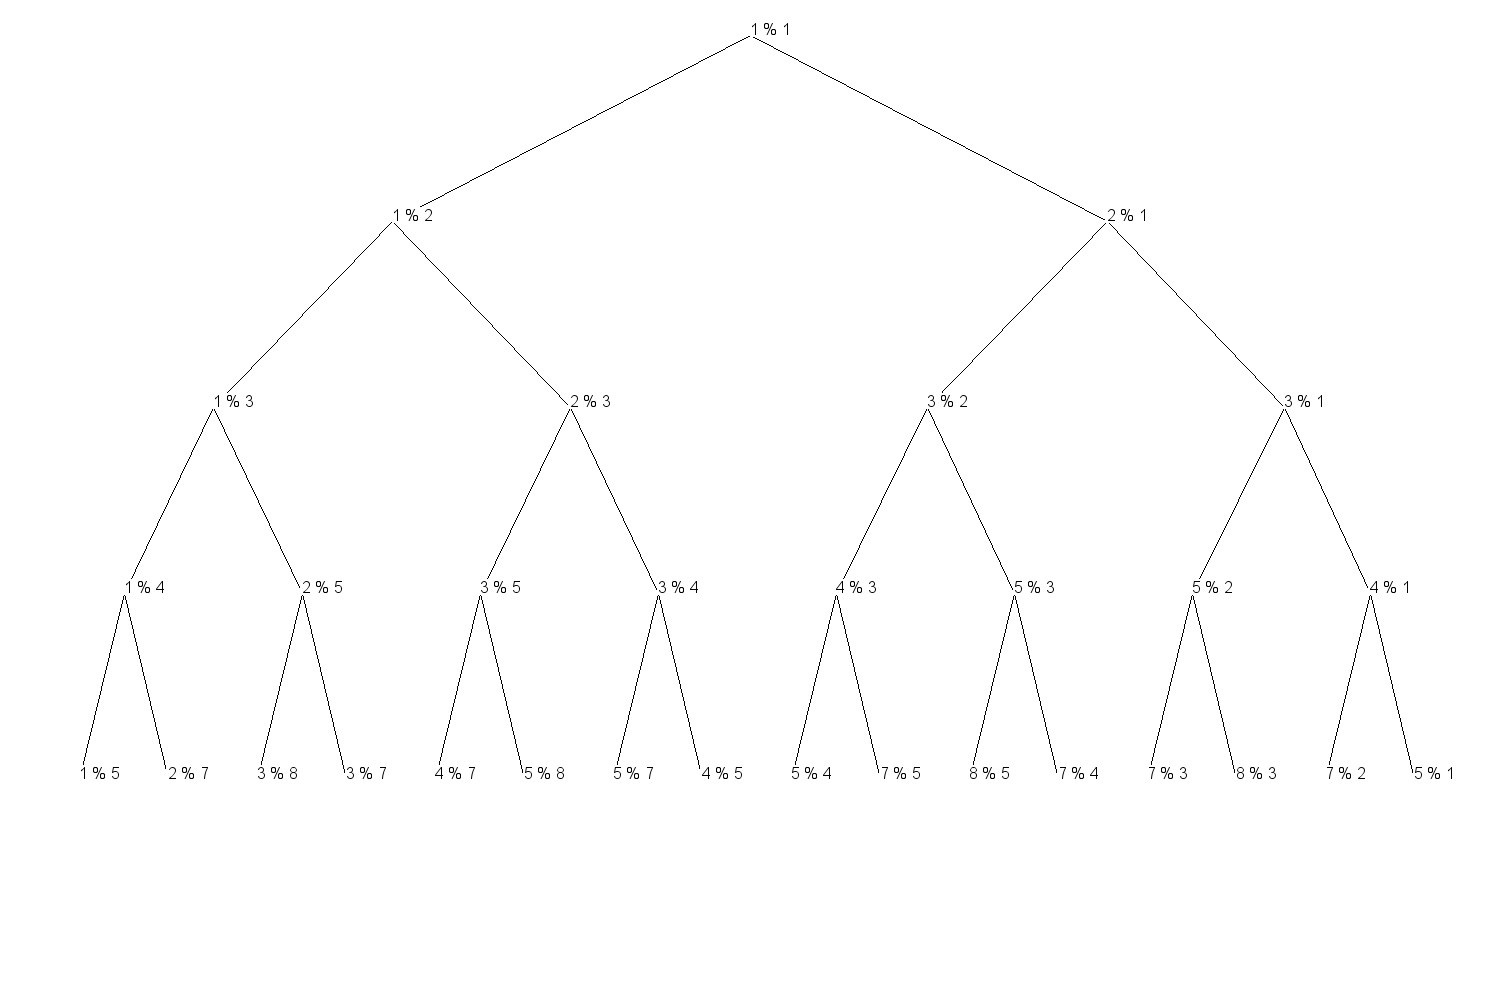
\includegraphics[width=\textwidth]{src/c06/sterb7}
%\end{center}

As you can see at once, this tree has many properties
in common with the Calkin-Wilf tree.
First and trivially, the left kid of a node $k$ is less
than $k$ and the right kid of the same node is greater than $k$.
The left-most branch of the tree contains all fractions
with 1 in the numerator like
$\frac{1}{1},
 \frac{1}{2},
 \frac{1}{3},
 \frac{1}{4}$ and so on.
The right-most branch contains the integers 
$\frac{1}{1},
 \frac{2}{1},
 \frac{3}{1},
 \frac{4}{1}$ and so on.

Furthermore, the product of each generation is 1.
For instance,
$\frac{1}{1} = 1$,
$\frac{1}{2} \times \frac{2}{1} = 1$,
$\frac{1}{3} \times \frac{2}{3} \times
 \frac{3}{2} \times \frac{3}{1} = 1$ and so on.
In fact, we see in each generation the same fractions
we would also see in the Calkin-Wilf tree.
The order of the fraction, however, is different.
More precisely, the order of the inner fractions
differs, since, as we have seen, 
the left-most and right-most numbers are the same.

We could hence ask the obvious question:
how can we permute the generations of the Stern-Brocot tree
to obtain the generations of the Calkin-Wilf tree and vice versa?
Let us look at an example.
The $4^{th}$ generation of the Calkin-Wilf tree is\\
\ensuremath{\Varid{getKids}\;\mathrm{4}\;(\Varid{calWiTree}\;\mathrm{4}\;(\Conid{Q}\;\mathrm{1}\;\mathrm{1}))}: 

\[
\frac{1}{4},
\frac{4}{3},
\frac{3}{5},
\frac{5}{2},
\frac{2}{5},
\frac{5}{3},
\frac{3}{4},
\frac{4}{1}.
\]

The $4^{th}$ generation of the Stern-Brocot tree is\\
\ensuremath{\Varid{getKids}\;\mathrm{4}\;(\Varid{sterbroctree}\;\mathrm{4})}: 

\[
\frac{1}{4},
\frac{2}{5},
\frac{3}{5},
\frac{3}{4},
\frac{4}{3},
\frac{5}{3},
\frac{5}{2},
\frac{4}{1}.
\]

We see that only some fractions changed their places
and the changes are all direct swaps, such that
the second position in the Calkin-Wilf tree changed with
the fifth position and
the fourth position changed with the seventh position.
The other positions, the first, third, sixth and eighth,
remain in their place. We could describe this in 
cyclic notation, using indexes from 0 -- 7 
for the eight positions:

\[
(1,4)(3,6).
\]

In other words,
we represent the generations as arrays with indexes 0 -- 7:

\begin{center}
\begingroup
\renewcommand{\arraystretch}{1.5}
\begin{tabular}{|c|c|c|c|c|c|c|c|c|}\hline
             & 0             & 1             & 2             & 3             & 4             & 5             & 6             & 7 \\\hline\hline
Calkin-Wilf  & $\frac{1}{4}$ & $\frac{4}{3}$ & $\frac{3}{5}$ & $\frac{5}{2}$ & $\frac{2}{5}$ & $\frac{5}{3}$ & $\frac{3}{4}$ & $\frac{4}{1}$\\\hline
Stern-Brocot & $\frac{1}{4}$ & $\frac{2}{5}$ & $\frac{3}{5}$ & $\frac{3}{4}$ & $\frac{4}{3}$ & $\frac{5}{3}$ & $\frac{5}{2}$ & $\frac{4}{1}$\\\hline
\end{tabular}
\endgroup
\end{center}

So, what is so special about the indexes 1, 3, 4 and 6
that distinguishes them from the indexes 0, 2, 5 and 7?
When we represent these numbers in binary format with
leading zeros, so that all binary numbers have the same length, we have

\begin{center}
\begin{tabular}{|c|c|c|c|c|c|c|c|}\hline
0    & 1   & 2    & 3   & 4   & 5   & 6   & 7 \\\hline\hline
000  & 001 & 010  & 011 & 100 & 101 & 110 & 111\\\hline
\end{tabular}
\end{center}

When we look at the indexes whose fractions do not change,
we see one property that they all have in common:
they are all symmetric. That is, when we reverse the bit strings,
we still have the same number.
$0 = 000$ reversed is still $000 = 0$;
$2 = 010$ reversed is still $010 = 2$;
$5 = 101$ reversed is still $101 = 5$ and
$7 = 111$ reversed is still $111 = 7$.
$1 = 001$ reversed, however, is $100 = 4$ and vice versa and
$3 = 011$ reversed is $110 = 6$.
This corresponds exactly 
to the permutation $(1,4)(3,6)$
and is an instance of a bit-reversal permutation.

Let us try to implement the bit-reversal permutation.
First we implement the bit-reverse of the indexes.
To do so, we first need to convert the decimal index
into a binary number; then we add zeros in front of all
binary numbers that are shorter
than the greatest number; then we simply
reverse the lists of binary digits, remove the leading
zeros and convert back to decimal numbers.
This can be nicely expressed by the function

\begin{minipage}{\textwidth}
\begingroup\par\noindent\advance\leftskip\mathindent\(
\begin{pboxed}\SaveRestoreHook
\column{B}{@{}>{\hspre}l<{\hspost}@{}}%
\column{3}{@{}>{\hspre}l<{\hspost}@{}}%
\column{15}{@{}>{\hspre}l<{\hspost}@{}}%
\column{25}{@{}>{\hspre}l<{\hspost}@{}}%
\column{47}{@{}>{\hspre}c<{\hspost}@{}}%
\column{47E}{@{}l@{}}%
\column{E}{@{}>{\hspre}l<{\hspost}@{}}%
\>[3]{}\Varid{bitrev}\mathbin{::}\Conid{Int}\to \Conid{Int}\to \Conid{Int}{}\<[E]%
\\
\>[3]{}\Varid{bitrev}\;\Varid{x}\mathrel{=}{}\<[15]%
\>[15]{}\Varid{fromIntegral}\mathbin{\circ}\Varid{fromBinary}{}\<[47]%
\>[47]{}\mathbin{\circ}{}\<[47E]%
\\
\>[15]{}\Varid{cleanz}\mathbin{\circ}{}\<[25]%
\>[25]{}\Varid{reverse}\mathbin{\circ}\Varid{fillup}\;\Varid{x}\;\mathrm{0}{}\<[47]%
\>[47]{}\mathbin{\circ}{}\<[47E]%
\\
\>[15]{}\Varid{toBinary}\mathbin{\circ}\Varid{fromIntegral}{}\<[E]%
\ColumnHook
\end{pboxed}
\)\par\noindent\endgroup\resethooks
\end{minipage}

where \ensuremath{\Varid{fillup}} is defined as

\begin{minipage}{\textwidth}
\begingroup\par\noindent\advance\leftskip\mathindent\(
\begin{pboxed}\SaveRestoreHook
\column{B}{@{}>{\hspre}l<{\hspost}@{}}%
\column{3}{@{}>{\hspre}l<{\hspost}@{}}%
\column{18}{@{}>{\hspre}c<{\hspost}@{}}%
\column{18E}{@{}l@{}}%
\column{21}{@{}>{\hspre}l<{\hspost}@{}}%
\column{37}{@{}>{\hspre}l<{\hspost}@{}}%
\column{E}{@{}>{\hspre}l<{\hspost}@{}}%
\>[3]{}\Varid{fillup}\mathbin{::}\Conid{Int}\to \Conid{Int}\to [\mskip1.5mu \Conid{Int}\mskip1.5mu]\to [\mskip1.5mu \Conid{Int}\mskip1.5mu]{}\<[E]%
\\
\>[3]{}\Varid{fillup}\;\Varid{i}\;\Varid{z}\;\Varid{is}{}\<[18]%
\>[18]{}\mid {}\<[18E]%
\>[21]{}\Varid{length}\;\Varid{is}\equiv \Varid{i}{}\<[37]%
\>[37]{}\mathrel{=}\Varid{is}{}\<[E]%
\\
\>[18]{}\mid {}\<[18E]%
\>[21]{}\Varid{otherwise}{}\<[37]%
\>[37]{}\mathrel{=}\Varid{fillup}\;\Varid{i}\;\Varid{z}\;(\Varid{z}\mathbin{:}\Varid{is}){}\<[E]%
\ColumnHook
\end{pboxed}
\)\par\noindent\endgroup\resethooks
\end{minipage}

and \ensuremath{\Varid{cleanz}} as 

\begin{minipage}{\textwidth}
\begingroup\par\noindent\advance\leftskip\mathindent\(
\begin{pboxed}\SaveRestoreHook
\column{B}{@{}>{\hspre}l<{\hspost}@{}}%
\column{3}{@{}>{\hspre}l<{\hspost}@{}}%
\column{18}{@{}>{\hspre}l<{\hspost}@{}}%
\column{E}{@{}>{\hspre}l<{\hspost}@{}}%
\>[3]{}\Varid{cleanz}\mathbin{::}[\mskip1.5mu \Conid{Int}\mskip1.5mu]\to [\mskip1.5mu \Conid{Int}\mskip1.5mu]{}\<[E]%
\\
\>[3]{}\Varid{cleanz}\;[\mskip1.5mu \mskip1.5mu]{}\<[18]%
\>[18]{}\mathrel{=}[\mskip1.5mu \mskip1.5mu]{}\<[E]%
\\
\>[3]{}\Varid{cleanz}\;[\mskip1.5mu \mathrm{0}\mskip1.5mu]{}\<[18]%
\>[18]{}\mathrel{=}[\mskip1.5mu \mathrm{0}\mskip1.5mu]{}\<[E]%
\\
\>[3]{}\Varid{cleanz}\;(\mathrm{0}\mathbin{:}\Varid{is}){}\<[18]%
\>[18]{}\mathrel{=}\Varid{cleanz}\;\Varid{is}{}\<[E]%
\\
\>[3]{}\Varid{cleanz}\;\Varid{is}{}\<[18]%
\>[18]{}\mathrel{=}\Varid{is}{}\<[E]%
\ColumnHook
\end{pboxed}
\)\par\noindent\endgroup\resethooks
\end{minipage}

To apply this, we first have to calculate
the size of the greatest number in our set
in binary format. If we assume that we have
a list of consecutive numbers from $0\dots n-1$,
then the size of the greatest number is just
$\log_2 n$, the binary logarithm of $n$.
For $n=8$, for instance, this is 3.
With this out of the way, we can define
a bit reversal of the indexes of any set \ensuremath{[\mskip1.5mu \Varid{a}\mskip1.5mu]} as:

\begin{minipage}{\textwidth}
\begingroup\par\noindent\advance\leftskip\mathindent\(
\begin{pboxed}\SaveRestoreHook
\column{B}{@{}>{\hspre}l<{\hspost}@{}}%
\column{3}{@{}>{\hspre}l<{\hspost}@{}}%
\column{19}{@{}>{\hspre}l<{\hspost}@{}}%
\column{23}{@{}>{\hspre}l<{\hspost}@{}}%
\column{24}{@{}>{\hspre}l<{\hspost}@{}}%
\column{27}{@{}>{\hspre}l<{\hspost}@{}}%
\column{E}{@{}>{\hspre}l<{\hspost}@{}}%
\>[3]{}\Varid{idxbitrev}\mathbin{::}[\mskip1.5mu \Varid{a}\mskip1.5mu]\to [\mskip1.5mu \Conid{Int}\mskip1.5mu]{}\<[E]%
\\
\>[3]{}\Varid{idxbitrev}\;\Varid{xs}\mathrel{=}{}\<[19]%
\>[19]{}\mathbf{let}\;{}\<[24]%
\>[24]{}\Varid{l}{}\<[27]%
\>[27]{}\mathrel{=}\Varid{fromIntegral}\mathbin{\$}\Varid{length}\;\Varid{xs}{}\<[E]%
\\
\>[24]{}\Varid{x}{}\<[27]%
\>[27]{}\mathrel{=}\Varid{round}\mathbin{\$}\Varid{logBase}\;\mathrm{2}\;(\Varid{fromIntegral}\;\Varid{l}){}\<[E]%
\\
\>[19]{}\mathbf{in}\;{}\<[23]%
\>[23]{}[\mskip1.5mu \Varid{bitrev}\;\Varid{x}\;\Varid{i}\mid \Varid{i}\leftarrow [\mskip1.5mu \mathrm{0}\mathinner{\ldotp\ldotp}\Varid{l}\mathbin{-}\mathrm{1}\mskip1.5mu]\mskip1.5mu]{}\<[E]%
\ColumnHook
\end{pboxed}
\)\par\noindent\endgroup\resethooks
\end{minipage}

and use this function to permute the original input list:

\begin{minipage}{\textwidth}
\begingroup\par\noindent\advance\leftskip\mathindent\(
\begin{pboxed}\SaveRestoreHook
\column{B}{@{}>{\hspre}l<{\hspost}@{}}%
\column{3}{@{}>{\hspre}l<{\hspost}@{}}%
\column{5}{@{}>{\hspre}l<{\hspost}@{}}%
\column{12}{@{}>{\hspre}l<{\hspost}@{}}%
\column{26}{@{}>{\hspre}l<{\hspost}@{}}%
\column{E}{@{}>{\hspre}l<{\hspost}@{}}%
\>[3]{}\Varid{bitreverse}\mathbin{::}[\mskip1.5mu \Varid{a}\mskip1.5mu]\to [\mskip1.5mu \Varid{a}\mskip1.5mu]{}\<[E]%
\\
\>[3]{}\Varid{bitreverse}\;\Varid{xs}\mathrel{=}\Varid{go}\;\Varid{xs}\;(\Varid{idxbitrev}\;\Varid{xs}){}\<[E]%
\\
\>[3]{}\hsindent{2}{}\<[5]%
\>[5]{}\mathbf{where}\;{}\<[12]%
\>[12]{}\Varid{go}\;\anonymous \;[\mskip1.5mu \mskip1.5mu]{}\<[26]%
\>[26]{}\mathrel{=}[\mskip1.5mu \mskip1.5mu]{}\<[E]%
\\
\>[12]{}\Varid{go}\;\Varid{zs}\;(\Varid{p}\mathbin{:}\Varid{ps}){}\<[26]%
\>[26]{}\mathrel{=}\Varid{zs}\mathbin{!!}\Varid{p}\mathbin{:}\Varid{go}\;\Varid{zs}\;\Varid{ps}{}\<[E]%
\ColumnHook
\end{pboxed}
\)\par\noindent\endgroup\resethooks
\end{minipage}

Applied on the list \ensuremath{[\mskip1.5mu \mathrm{0},\mathrm{1},\mathrm{2},\mathrm{3},\mathrm{4},\mathrm{5},\mathrm{6}\mskip1.5mu]},
we see exactly the $(1,4)(3,6)$ permutation
we saw above, namely \ensuremath{[\mskip1.5mu \mathrm{0},\mathrm{4},\mathrm{2},\mathrm{6},\mathrm{1},\mathrm{5},\mathrm{3}\mskip1.5mu]}.
Applied on a generation from the Calkin-Wilf tree,
we see the corresponding generation from the 
Stern-Brocot tree. 
Let \ensuremath{\Varid{t}\mathrel{=}\Varid{calWiTree}\;(\mathbin{-}\mathrm{1})\;(\mathrm{1}\mathbin{\%}\mathrm{1})},
we see for 

\begin{center}
\begingroup
\renewcommand{\arraystretch}{1.5}
\begin{tabular}{|c|c|}\hline
\ensuremath{\Varid{getKids}\;\mathrm{3}\;\Varid{t}} & 
$\frac{1}{3},
 \frac{3}{2},
 \frac{2}{3},
 \frac{3}{1}$ \\\hline
\ensuremath{\Varid{bitreverse}\;(\Varid{getKids}\;\mathrm{3}\;\Varid{t})} &
$\frac{1}{3},
 \frac{2}{3},
 \frac{3}{2},
 \frac{3}{1}$\\\hline
\ensuremath{\Varid{getKids}\;\mathrm{4}\;\Varid{t}} & 
$\frac{1}{4},
 \frac{4}{3},
 \frac{3}{5},
 \frac{5}{2},
 \frac{2}{5},
 \frac{5}{3},
 \frac{3}{4}, 
 \frac{4}{1}$ \\\hline
\ensuremath{\Varid{bitreverse}\;(\Varid{getKids}\;\mathrm{4}\;\Varid{t})} &
$\frac{1}{4},
 \frac{2}{5},
 \frac{3}{5},
 \frac{3}{4},
 \frac{4}{3},
 \frac{5}{3},
 \frac{5}{2},
 \frac{4}{1}$\\\hline
\end{tabular}
\endgroup
\end{center}

Since the generations of the Stern-Brocot tree
are nothing but permutations of the Calkin-Wilf tree, we
can derive a sequence from the Stern-Brocot tree
that lists all rational numbers.
We create this sequence in exaclty the same way
we did for the CalkinWilf tree, namely

\begin{minipage}{\textwidth}
\begingroup\par\noindent\advance\leftskip\mathindent\(
\begin{pboxed}\SaveRestoreHook
\column{B}{@{}>{\hspre}l<{\hspost}@{}}%
\column{3}{@{}>{\hspre}l<{\hspost}@{}}%
\column{5}{@{}>{\hspre}l<{\hspost}@{}}%
\column{E}{@{}>{\hspre}l<{\hspost}@{}}%
\>[3]{}\Varid{enumQsb}\mathbin{::}[\mskip1.5mu \Conid{Ratio}\mskip1.5mu]{}\<[E]%
\\
\>[3]{}\Varid{enumQsb}\mathrel{=}\Varid{go}\;\mathrm{1}\mathbin{\$}\Varid{sterbrocTree}\;(\mathbin{-}\mathrm{1}){}\<[E]%
\\
\>[3]{}\hsindent{2}{}\<[5]%
\>[5]{}\mathbf{where}\;\Varid{go}\;\Varid{i}\;\Varid{t}\mathrel{=}\Varid{getKids}\;\Varid{i}\;\Varid{t}\plus \Varid{go}\;(\Varid{i}\mathbin{+}\mathrm{1})\;\Varid{t}{}\<[E]%
\ColumnHook
\end{pboxed}
\)\par\noindent\endgroup\resethooks
\end{minipage}\ignore{$}

The numerators of the sequence derived in this way
from the Calkin-Wilf tree equal the well-known Stern sequence.
Is there another well-known sequence that is equivalent
to the numerators of the Stern-Brocot tree sequence?
Let us ask the On-line Encyclopedia with the first segment
of that sequence generated by \ensuremath{\Varid{map}\;\Varid{numerator}\;(\Varid{take}\;\mathrm{20}\;\Varid{enumQsb})}:

\[
1,1,2,1,2,3,3,1,2,3,3,4,5,5,4,1,2,3,3,4,5,5,4,5,7.
\]

The Encyclopedia tells us that this is the numerators of
the \term{Farey sequence}.
This sequence, named for British geologist 
John Farey (1766 -- 1826), has a lot of remarkable properties.
The Farey sequence of $n$ lists all fractions 
in canoncial form between 0 and 1,
usually included, with a denominator less or equal than $n$.
For instance, the Farey sequence of 1, designated $F_1$ just contains
$0,1$; $F_2$ contains $0,\frac{1}{2},1$;
$F_3$ contains $0,\frac{1}{3},\frac{2}{3},1$ and so on.

A direct way to implement this could be to combine all numbers
from $0\dots n$ in the numerator with all numbers $1\dots n$
in the denominator that are smaller than 1 and to sort and \ensuremath{\Varid{nub}}
the resulting list, like this:

\begin{minipage}{\textwidth}
\begingroup\par\noindent\advance\leftskip\mathindent\(
\begin{pboxed}\SaveRestoreHook
\column{B}{@{}>{\hspre}l<{\hspost}@{}}%
\column{3}{@{}>{\hspre}l<{\hspost}@{}}%
\column{27}{@{}>{\hspre}l<{\hspost}@{}}%
\column{E}{@{}>{\hspre}l<{\hspost}@{}}%
\>[3]{}\Varid{farey2}\mathbin{::}\Conid{Natural}\to [\mskip1.5mu \Conid{Ratio}\mskip1.5mu]{}\<[E]%
\\
\>[3]{}\Varid{farey2}\;\Varid{n}\mathrel{=}\Varid{sort}\;(\Varid{nub}\mathbin{\$}{}\<[27]%
\>[27]{}\Varid{filter}\;(\leq \mathrm{1})\mathbin{\$}{}\<[E]%
\\
\>[27]{}\Varid{concatMap}\;(\lambda \Varid{x}\to \Varid{map}\;(\Varid{x}\mathbin{\%})\;[\mskip1.5mu \mathrm{1}\mathinner{\ldotp\ldotp}\Varid{n}\mskip1.5mu])\;[\mskip1.5mu \mathrm{0}\mathinner{\ldotp\ldotp}\Varid{n}\mskip1.5mu]){}\<[E]%
\ColumnHook
\end{pboxed}
\)\par\noindent\endgroup\resethooks
\end{minipage}

With this approach, we create a lot of fractions
that we do not need and that we filter out again afterwards.
A more interesting approach, also in the light of the topic
of this section, is the following:

\begin{minipage}{\textwidth}
\begingroup\par\noindent\advance\leftskip\mathindent\(
\begin{pboxed}\SaveRestoreHook
\column{B}{@{}>{\hspre}l<{\hspost}@{}}%
\column{3}{@{}>{\hspre}l<{\hspost}@{}}%
\column{5}{@{}>{\hspre}l<{\hspost}@{}}%
\column{12}{@{}>{\hspre}l<{\hspost}@{}}%
\column{20}{@{}>{\hspre}c<{\hspost}@{}}%
\column{20E}{@{}l@{}}%
\column{23}{@{}>{\hspre}l<{\hspost}@{}}%
\column{28}{@{}>{\hspre}l<{\hspost}@{}}%
\column{E}{@{}>{\hspre}l<{\hspost}@{}}%
\>[3]{}\Varid{farey}\mathbin{::}\Conid{Natural}\to [\mskip1.5mu \Conid{Ratio}\mskip1.5mu]{}\<[E]%
\\
\>[3]{}\Varid{farey}\;\Varid{n}\mathrel{=}\mathrm{0}\mathbin{:}\Varid{sort}\;(\Varid{go}\;\mathrm{1}\mathbin{\$}\Varid{sterbrocTree}\;(\mathbin{-}\mathrm{1})){}\<[E]%
\\
\>[3]{}\hsindent{2}{}\<[5]%
\>[5]{}\mathbf{where}\;{}\<[12]%
\>[12]{}\Varid{go}\;\Varid{k}\;\Varid{t}{}\<[20]%
\>[20]{}\mathrel{=}{}\<[20E]%
\>[23]{}\mathbf{let}\;{}\<[28]%
\>[28]{}\Varid{g}\mathrel{=}\Varid{getKids}\;\Varid{k}\;\Varid{t}{}\<[E]%
\\
\>[28]{}\Varid{l}\mathrel{=}\Varid{filter}\;\Varid{fltr}\;\Varid{g}{}\<[E]%
\\
\>[23]{}\mathbf{in}\;\mathbf{if}\;\Varid{null}\;\Varid{l}\;\mathbf{then}\;\Varid{l}\;\mathbf{else}\;\Varid{l}\plus \Varid{go}\;(\Varid{k}\mathbin{+}\mathrm{1})\;\Varid{t}{}\<[E]%
\\
\>[12]{}\Varid{fltr}\;\Varid{k}{}\<[20]%
\>[20]{}\mathrel{=}{}\<[20E]%
\>[23]{}\Varid{k}\leq \mathrm{1}\mathrel{\wedge}\Varid{n}\geq \Varid{denominator}\;\Varid{k}{}\<[E]%
\ColumnHook
\end{pboxed}
\)\par\noindent\endgroup\resethooks
\end{minipage}\ignore{$}

Here, we iterate over the generations of the Stern-Brocot tree
removing the fractions that are greater than 1 or have a denominator
greater n. When we do not get results anymore, \ie\ all denominators
are greater than $n$, we are done.

Let us try this algorithm on some numbers:

\begin{equation}
F_4 = \left\lbrace 0, 
\frac{1}{4}, 
\frac{1}{3}, 
\frac{1}{2}, 
\frac{2}{3}, 
\frac{3}{4}, 
1\right\rbrace
\end{equation}
\begin{equation}
F_5 = \left\lbrace 0, 
\frac{1}{5}, 
\frac{1}{4}, 
\frac{1}{3}, 
\frac{2}{5}, 
\frac{1}{2}, 
\frac{3}{5}, 
\frac{2}{3}, 
\frac{3}{4}, 
\frac{4}{5}, 
1\right\rbrace
\end{equation}
\begin{equation}
F_6 = \left\lbrace 0, 
\frac{1}{6}, 
\frac{1}{5}, 
\frac{1}{4}, 
\frac{1}{3}, 
\frac{2}{5}, 
\frac{1}{2}, 
\frac{3}{5}, 
\frac{2}{3}, 
\frac{3}{4}, 
\frac{4}{5}, 
\frac{5}{6}, 
1\right\rbrace
\end{equation}

We see some interesting properties.
First and this should be obvious,
we see $n$ as a denominator in sequence $F_n$ exaclty
$\varphi(n)$ times.
For $F_6$, for instance, we could create the fractions
$\frac{1}{6}$, 
$\frac{2}{6}$, 
$\frac{3}{6}$, 
$\frac{4}{6}$ and
$\frac{5}{6}$.
The fractions $\frac{2}{6}\dots\frac{4}{6}$, however,
are not in canonical form, since the numerators $2\dots 4$ 
all share divisors with 6. 
Since there are $\varphi(n)$ numerators
that do not share divisors with $n$,
there are only $\varphi(n)$ fractions less than 1
whith $n$ in the denominator. 

Another property is that, for two consecutive fractions
in the Farey sequence,
$\frac{a}{b}$ and $\frac{c}{d}$,
the cross products
$ad$ and $cb$ are consecutive integers.
In again $F_6$, 
for the fractions $\frac{1}{6}$ and $\frac{1}{5}$,
the cross products, trivially, are 5 and 6.
More interesting are 
the fractions $\frac{3}{5}$ and $\frac{2}{3}$ whose
cross products are $3\times 3 = 9$ and $5 \times 2 = 10$.

Even further, for any three consecutive fractions
in a Farey sequence, the middle one, called the mediant fraction,
can be calculated from the outer ones as
$\frac{a}{b}, \frac{a+c}{b+d}, \frac{c}{d}$.
For instance in $F_6$: 

\begin{equation}
 \frac{1+1}{6+4} = \frac{2}{10} = \frac{1}{5},
\end{equation}
\begin{equation}
 \frac{2+3}{5+5} = \frac{5}{10} = \frac{1}{2}
\end{equation}
and
\begin{equation}
 \frac{3+5}{4+6} = \frac{8}{10} = \frac{4}{5}.
\end{equation}

This property can be used to compute $F_{n+1}$ from $F_n$.
We just have to insert those mediant fractions 
of two consecutive fractions in $F_n$, for which
the denominator is $n+1$.
In $F_6$ we would insert

\[
\frac{0+1}{1+6},
\frac{1+1}{4+3},
\frac{2+1}{5+2},
\frac{1+3}{2+5},
\frac{2+3}{3+4},
\frac{5+1}{6+1}
\]

resulting in

\begin{equation}
F_7 = \left\lbrace 0, 
\frac{1}{7}, 
\frac{1}{6}, 
\frac{1}{5}, 
\frac{1}{4}, 
\frac{2}{7}, 
\frac{1}{3}, 
\frac{2}{5}, 
\frac{3}{7}, 
\frac{1}{2}, 
\frac{4}{7}, 
\frac{3}{5}, 
\frac{2}{3}, 
\frac{5}{7}, 
\frac{3}{4}, 
\frac{4}{5}, 
\frac{5}{6}, 
\frac{6}{7}, 
1\right\rbrace
\end{equation}

We can implement this as

\begin{minipage}{\textwidth}
\begingroup\par\noindent\advance\leftskip\mathindent\(
\begin{pboxed}\SaveRestoreHook
\column{B}{@{}>{\hspre}l<{\hspost}@{}}%
\column{3}{@{}>{\hspre}l<{\hspost}@{}}%
\column{5}{@{}>{\hspre}l<{\hspost}@{}}%
\column{16}{@{}>{\hspre}l<{\hspost}@{}}%
\column{19}{@{}>{\hspre}l<{\hspost}@{}}%
\column{20}{@{}>{\hspre}l<{\hspost}@{}}%
\column{21}{@{}>{\hspre}l<{\hspost}@{}}%
\column{24}{@{}>{\hspre}c<{\hspost}@{}}%
\column{24E}{@{}l@{}}%
\column{27}{@{}>{\hspre}l<{\hspost}@{}}%
\column{47}{@{}>{\hspre}l<{\hspost}@{}}%
\column{E}{@{}>{\hspre}l<{\hspost}@{}}%
\>[3]{}\Varid{nxtFarey}\mathbin{::}\Conid{Natural}\to [\mskip1.5mu \Conid{Ratio}\mskip1.5mu]\to [\mskip1.5mu \Conid{Ratio}\mskip1.5mu]{}\<[E]%
\\
\>[3]{}\Varid{nxtFarey}\;\Varid{n}\;[\mskip1.5mu \mskip1.5mu]{}\<[19]%
\>[19]{}\mathrel{=}[\mskip1.5mu \mskip1.5mu]{}\<[E]%
\\
\>[3]{}\Varid{nxtFarey}\;\Varid{n}\;[\mskip1.5mu \Varid{r}\mskip1.5mu]{}\<[19]%
\>[19]{}\mathrel{=}[\mskip1.5mu \Varid{r}\mskip1.5mu]{}\<[E]%
\\
\>[3]{}\Varid{nxtFarey}\;\Varid{n}\;(\Varid{a}\mathbin{:}\Varid{b}\mathbin{:}\Varid{rs}){}\<[24]%
\>[24]{}\mid {}\<[24E]%
\>[27]{}\Varid{denominator}\;\Varid{a}\mathbin{+}{}\<[E]%
\\
\>[27]{}\Varid{denominator}\;\Varid{b}\equiv \Varid{n}{}\<[47]%
\>[47]{}\mathrel{=}\Varid{nxtFarey}\;\Varid{n}\;(\Varid{a}\mathbin{:}\Varid{x}\mathbin{:}\Varid{b}\mathbin{:}\Varid{rs}){}\<[E]%
\\
\>[24]{}\mid {}\<[24E]%
\>[27]{}\Varid{otherwise}{}\<[47]%
\>[47]{}\mathrel{=}\Varid{a}\mathbin{:}\Varid{nxtFarey}\;\Varid{n}\;(\Varid{b}\mathbin{:}\Varid{rs}){}\<[E]%
\\
\>[3]{}\hsindent{2}{}\<[5]%
\>[5]{}\mathbf{where}\;\Varid{x}\mathrel{=}{}\<[16]%
\>[16]{}\mathbf{let}\;{}\<[21]%
\>[21]{}\Varid{n1}\mathrel{=}\Varid{numerator}\;\Varid{a}{}\<[E]%
\\
\>[21]{}\Varid{n2}\mathrel{=}\Varid{numerator}\;\Varid{b}{}\<[E]%
\\
\>[21]{}\Varid{d1}\mathrel{=}\Varid{denominator}\;\Varid{a}{}\<[E]%
\\
\>[21]{}\Varid{d2}\mathrel{=}\Varid{denominator}\;\Varid{b}{}\<[E]%
\\
\>[16]{}\mathbf{in}\;{}\<[20]%
\>[20]{}(\Varid{n1}\mathbin{+}\Varid{n2})\mathbin{\%}(\Varid{d1}\mathbin{+}\Varid{d2}){}\<[E]%
\ColumnHook
\end{pboxed}
\)\par\noindent\endgroup\resethooks
\end{minipage}
 
In fact, we can construct the Stern-Brocot tree
by means of mediant fractions. The outer fractions,
in this algorithm are the predecessors of the current node,
namely the direct predecessor and either the predecessor
of the predecessor or the sibling of that node.
For instance, the second node in the third generation
is $\frac{2}{3}$. Its kids are 
$\frac{3}{5}$ and $\frac{3}{4}$.
$\frac{3}{5}$ is $\frac{2+1}{3+2}$ and, thus,
the sum of $\frac{2}{3}$ and its predecessor;
$\frac{4}{3}$, however, is $\frac{2+1}{3+1}$
and, hence, the sum of the $\frac{2}{3}$ 
and the predecessor of its predecessor.

The question now is how to bootstrap this algorithm.
The root node, of course, does not have predecessors.
For this case, we imagine two predecessors, namely
the fractions $\frac{0}{1}$ and $\frac{1}{0}$,
the latter of which, of course, is not a proper fraction.
The assumption of such nodes, however, helps us derive
the outer branches, where, on the left side, the numerator
does not change, hence is constructed by addition with 0, and,
on the right side, the denominator does not change and is
likewise constructed by addition with 0.

We implement this as

\begin{minipage}{\textwidth}
\begingroup\par\noindent\advance\leftskip\mathindent\(
\begin{pboxed}\SaveRestoreHook
\column{B}{@{}>{\hspre}l<{\hspost}@{}}%
\column{3}{@{}>{\hspre}l<{\hspost}@{}}%
\column{29}{@{}>{\hspre}l<{\hspost}@{}}%
\column{30}{@{}>{\hspre}c<{\hspost}@{}}%
\column{30E}{@{}l@{}}%
\column{33}{@{}>{\hspre}l<{\hspost}@{}}%
\column{38}{@{}>{\hspre}l<{\hspost}@{}}%
\column{42}{@{}>{\hspre}l<{\hspost}@{}}%
\column{44}{@{}>{\hspre}l<{\hspost}@{}}%
\column{54}{@{}>{\hspre}l<{\hspost}@{}}%
\column{E}{@{}>{\hspre}l<{\hspost}@{}}%
\>[3]{}\Varid{mSterbroctree}\mathbin{::}\Conid{Zahl}\to {}\<[29]%
\>[29]{}\Conid{Natural}\to \Conid{Natural}\to {}\<[E]%
\\
\>[29]{}\Conid{Natural}\to \Conid{Natural}\to \Conid{Ratio}\to \Conid{Tree}\;\Conid{Ratio}{}\<[E]%
\\
\>[3]{}\Varid{mSterbroctree}\;\mathrm{0}\;\anonymous \;\anonymous \;\anonymous \;\anonymous \;\Varid{r}{}\<[30]%
\>[30]{}\mathrel{=}{}\<[30E]%
\>[33]{}\Conid{Node}\;\Varid{r}\;[\mskip1.5mu \mskip1.5mu]{}\<[E]%
\\
\>[3]{}\Varid{mSterbroctree}\;\Varid{n}\;\Varid{a}\;\Varid{b}\;\Varid{c}\;\Varid{d}\;\Varid{r}{}\<[30]%
\>[30]{}\mathrel{=}{}\<[30E]%
\>[33]{}\mathbf{let}\;{}\<[38]%
\>[38]{}\Varid{rn}{}\<[42]%
\>[42]{}\mathrel{=}\Varid{numerator}\;\Varid{r}{}\<[E]%
\\
\>[38]{}\Varid{rd}{}\<[42]%
\>[42]{}\mathrel{=}\Varid{denominator}\;\Varid{r}{}\<[E]%
\\
\>[38]{}\Varid{k1}{}\<[42]%
\>[42]{}\mathrel{=}(\Varid{a}\mathbin{+}\Varid{rn})\mathbin{\%}(\Varid{b}\mathbin{+}\Varid{rd}){}\<[E]%
\\
\>[38]{}\Varid{k2}{}\<[42]%
\>[42]{}\mathrel{=}(\Varid{c}\mathbin{+}\Varid{rn})\mathbin{\%}(\Varid{d}\mathbin{+}\Varid{rd}){}\<[E]%
\\
\>[33]{}\mathbf{in}\;{}\<[38]%
\>[38]{}\mathbf{if}\;\Varid{k1}\mathbin{<}\Varid{k2}{}\<[E]%
\\
\>[38]{}\mathbf{then}\;{}\<[44]%
\>[44]{}\Conid{Node}\;\Varid{r}\;[\mskip1.5mu {}\<[54]%
\>[54]{}\Varid{mSterbroctree}\;(\Varid{n}\mathbin{-}\mathrm{1})\;\Varid{a}\;\Varid{b}\;\Varid{rn}\;\Varid{rd}\;\Varid{k1},{}\<[E]%
\\
\>[54]{}\Varid{mSterbroctree}\;(\Varid{n}\mathbin{-}\mathrm{1})\;\Varid{c}\;\Varid{d}\;\Varid{rn}\;\Varid{rd}\;\Varid{k2}\mskip1.5mu]{}\<[E]%
\\
\>[38]{}\mathbf{else}\;{}\<[44]%
\>[44]{}\Conid{Node}\;\Varid{r}\;[\mskip1.5mu {}\<[54]%
\>[54]{}\Varid{mSterbroctree}\;(\Varid{n}\mathbin{-}\mathrm{1})\;\Varid{c}\;\Varid{d}\;\Varid{rn}\;\Varid{rd}\;\Varid{k2},{}\<[E]%
\\
\>[54]{}\Varid{mSterbroctree}\;(\Varid{n}\mathbin{-}\mathrm{1})\;\Varid{a}\;\Varid{b}\;\Varid{rn}\;\Varid{rd}\;\Varid{k1}\mskip1.5mu]{}\<[E]%
\ColumnHook
\end{pboxed}
\)\par\noindent\endgroup\resethooks
\end{minipage}

Note that we have to use two pairs of natural numbers
instead of two fractions to encode the predecessors.
This is because we have to represent the imagined
predecessor $\frac{1}{0}$, which is not a proper fraction.
Finally, we check for the smaller of the resulting numbers
$k_1$ and $k_2$ to make sure that the smaller one 
always goes to the left and the greater to the right.
This implementation now gives exactly the same tree
as the implementation using continued fractions
introduced at the beginning of the section.

\section{p-adic Numbers} 
\section{Real Factorials}
\section{The Continuum}
\section{Review of the Number Zoo}


\end{document}
